% プロジェクト学習中間報告書書式テンプレート ver.1.0 (iso-2022-jp)

% 両面印刷する場合は `openany' を削除する
\documentclass[openany,11pt,papersize]{jsbook}

% 報告書提出用スタイルファイル
%\usepackage[final]{funpro}%最終報告書
\usepackage[middle]{funpro}%中間報告書

% 画像ファイル (EPS, EPDF, PNG) を読み込むために
\usepackage[dvipdfmx]{graphicx,color}

% ここから -->
\usepackage{calc,ifthen}
\newcounter{hoge}
\newcommand{\fake}[1]{\whiledo{\thehoge<70}{#1\stepcounter{hoge}}%
  \setcounter{hoge}{0}}
% <-- ここまで 削除してもよい

\usepackage{here}

% 年度の指定
\thisYear{2015}

% プロジェクト名
\jProjectName{フィールドから創る地域・社会のためのスウィフトなアプリ開発}

% [簡易版のプロジェクト名]{正式なプロジェクト名}
% 欧文のプロジェクト名が極端に長い(2行を超える)場合は、短い記述を
% 任意引数として渡す。
%\eProjectName[Making Delicious curry]{How to make delicious curry of Hakodate}
\eProjectName{``Swift'' Application Development Based on Field Research}


% <プロジェクト番号>-<グループ名>
\ProjectNumber{3-C}

% グループ名
\jGroupName{教育系グループ}
\eGroupName{Education Group}

% プロジェクトリーダ
\ProjectLeader{1013220}{新保遥平}{Yohei~Shinpo}

% グループリーダ
\GroupLeader  {1013015}{中進吾}{Shingo~Naka}

% メンバー数
\SumOfMembers{5}
% グループメンバ
\GroupMember  {1}{1013130}{熊谷優斗}{Yuto~Kumagai}
\GroupMember  {2}{1013116}{皀勢也}{Seiya~Kurokome}
\GroupMember  {3}{1013220}{新保遥平}{Yohei~Shinpo}
\GroupMember  {4}{1013015}{中進吾}{Shingo~Naka}
\GroupMember  {5}{1013104}{矢吹渓悟}{Keigo~Yabuki}

% 指導教員
\jadvisor{伊藤恵,奥野拓,原田泰,木塚あゆみ,南部美砂子}
% 複数人数いる場合はカンマ(,)で区切る。カンマの前後に空白は入れない。
\eadvisor{Kei~Itou,Taku~Okuno,Yasushi~Harada,Ayumi~Kizuka,Misako~Nambu}

% 論文提出日
\jdate{2015年7月29日}
\edate{July~29, 2015}

%%%%%%%%%%%%%%%%%%%%%%%%%%%%%%%%%%%%%%%
\usepackage{graphicx}
%%%%%%%%%%%%%%%%%%%%%%%%%%%%%%%%%%%%%%%
\begin{document}
%
% 表紙
\maketitle

%前付け
\frontmatter

% 和文概要
\begin{jabstract} 
%\fake{ここに日本語の概要を書きます。}
 本プロジェクトは教育というフィールドを調査し、教育に関する問題を解決するアプリケーションを開発することを目的としている。

 各メンバーが教育に関わるアプリを考え、メンバーと担当教員にプレゼンテーションを行った。メンバー間では情報の共有を行い、担当教員からはレビューを受けた。その後、担当教員から受けたレビューを基にお互いにアイデアを広げ、テーマを1つに絞り込み中学生向けプログラミング入門アプリに決まった。%\テーマが決まった後、アプリの設計を行った。しかし、要件定義を固めずにアプリの設計を行ったため、一貫性のないアプリ設計になってしまった。そのため、要件定義を1からやり直すことになった。要件定義をやり直すことは、1度で終わらず何度も行った。その結果、中学校でプログラミングを学んだ人、興味を持った人を対象にしたゲームアプリというテーマに決めた。
%\現在日本の中学校では、2012年から中学校の技術家庭科でプログラミング教育が必修項目となっている。しかし、今の中学校のプログラミング教育ではソースコードを打ってプログラミングをするということを行っておらず、プログラミングの内容を深く取り上げていない。そこで、私たちは中学で学んだプログラミングと実際のプログラミングの間のプロセスを支援するゲームアプリを開発することを決めた。

 中間発表では、私たちが考えた提案をポスターにまとめ、ポスターセッションを行った。教員や他学生からの評価シートには「最終的なゴールは?」、「まだ内容が決まっていないので評価不能」、「既存のもとの比較がない」などの意見をいただき、もう1度要件定義を見直しアプリの設計をやり直す必要があることに気付かされた。

 後期は、夏休みにメンバー各自で調べてきた教育のアイデアを出し合い、後期のプロジェクトのテーマについて何度も話し合った。その結果、C言語を学んでいる大学生を対象としたC言語のWebアプリケーションの学習教材を開発するテーマに決めた。
 %\現在、C言語を学んでいる公立はこだて未来大学の学生とその講義を担当しているTA(Teaching Assistant)にヒアリング調査を行った。その結果、C言語の配列などの概念やアルゴリズムが分かっていないことが分かった。また、現在使われている講義資料を確認してみたところ、ほとんどが文字で構成されており、専門用語が多くあり、C言語を初めて学ぶ学生にとっては分かりにくい講義資料だと思った。そこで、私たちはこれらの課題を解決するためアニメーションで、概念やアルゴリズムを教えるWebアプリケーションを開発することを決めた。

 最終発表では、中間発表と同様に私たちが考えた提案をポスターにまとめ、ポスターセッションを行った。教員や他学生からの評価シートには「イメージがわくので、分かり易かったです」などの意見をいただき前期と比べて評価は高かった。一方で、「実際に1年生に使ってほしかった」、「他の班と比べてiOSアプリを作らなかったメリットを知りたい」などの意見をいただき、今後の改善点を見つけることができた。

 今後の展望としては、私たちが作成した提案物と酷似したソフトウェアが本学の2年次の科目である「アルゴリズムとデータ構造」の教科書の付属CDにあったため、そのソフトウェアとの差別化を図っていきたいと思う。また、ユーザーに評価していただくために本学の1年生やメタ学習センターに実際に使っていただきたいと思う。

% 和文キーワード
%\begin{jkeyword}
%キーワード1, キーワード2, キーワード3, キーワード4, キーワード5
%\end{jkeyword}
\bunseki{中進吾}
\end{jabstract}

%英語の概要
\begin{eabstract} 
%\fake{you should write your English abstract in one page. }
 This project is having for its object to investigate a field as education and develop the application useful for education.

 Each member considered the application of educating and presented members and teachers. We shared information among the members and received reviews from teachers. After those ideas was expanded each other and the theme was narrowed down to 1 based on the review we received from teachers. The theme was decided in programming guide application for junior high schoolll students.
%\After the theme was decided, the application was designed. But the design of application had inconsistent because the application was designed without making the requirement definition hard. Therefore we changed the requirement definition from one. We did not finish changing the requirement definition and went many times. As a result, it was decided in the theme as the game application that made the person who learned a programming at junior high school and interested people the subject.
%\Programming education is the compulsory item at technical and homemaking course of Japanese junior high school from 2012. But neither to hit source cord with programming education of the junior high school and program be being performed nor the contents of programming be taken up deeply now. So we have decided to develop the game application which supports process between the programming learned at junior high school and the actual programming.

 The proposition that we thought was gathered in a poster and a poster session was performed in the middle announcement. We received opinions of which ``what is last goal'', ``having no comparison it exists down'', ``the contents are not decided yet, so evaluation is impossible'' in an evaluation seat from teachers and other students, and the requirement definition was reconsidered again, and they made notice that it is necessary to redo design of an application.

 In the latter period, educational ideas that members found in the summer holidays was shared and we discussed theme of project many times. As a result, The theme was decided in Web application teaches C language for college students learning it.
%\We investigated Future University HAKODATE students learned C language and Teaching Assistant took the lecture now. As a result, we knew that they do not know array's concept of C language and algorithm. We think that the lecture material used was difficult for them because it was made of most characters and had professional words when we checked it. We decided that we made Web application teaches concept and algorithm in animation to resolve these problems.

 The proposition that we thought was gathered in a poster and a poster session was performed like the first term in the final announcement. We received opinions of which ``it is easy because I can imagine'' in an evaluation seat from teachers and other students, and the evaluation of the latter period was better than it of the first period. Also, we received opinions of which ``I hope this Web site was used by 1st grader'', ``Compared with other groups, I want to know the merit of not making iOS application'' and we knew the improvement points of future.

I would like to plan for differentiation with the software because the suggestion thing we made and software I resemble closely matched an accessory CD of the textbook of ``algorithm and data structure'' which is 2 grader of subject of the science as future's view. I would like to ask the user to use it for 1st grader of this college and the META learning center actually to estimate.
% 英文キーワード
%\begin{ekeyword}
%Keyrods1, Keyword2, Keyword3, Keyword4, Keyword5
%\end{ekeyword}
\bunseki{中進吾}
\end{eabstract}

\tableofcontents% 目次


\mainmatter% 本文のはじまり

\chapter{はじめに}
私たち教育系チームはこの1年間を通して、プログラミング教育という視点でアプリの開発を
行ってきた。自分たちのアプリでプログラミングを理解して楽しんでもらうという目的で
あった。私たちのグループでは前期から後期を通して幾度となく、アプリ案の変更があった。
前期ではSwift言語によるアプリ案を考えてきた。だが後期からはHTMLやProcessingを
用いたWebアプリケーションの開発に移行していった。
第2章から第6章までが前期の活動である。前期では、ユーザを意識したアプリ案が少なく自分たちの作りたいアプリ案を多く提案していた。また、実装まで進めた後でアプリのコンセプトの見直しなどが多くあった。そのため、アプリ案の再設計というのが前期の教育系の進捗であった。
第7章から第11章が後期の活動である。後期は前期の反省を踏まえ、アプリ案の提案に慎重に
なりすぎてしまい、アプリの実装に進むことができなかった。だが
最終成果発表会までには自分たちの納得のいく成果物を作ることができた。
\bunseki{新保遥平}

\chapter{前期の背景}
\section{世界と日本のプログラミング教育について}
現在、世界中でプログラミング教育の必要性が高まっている。政府が公教育としてプログラミングを取り入れている、または取り入れようとしている国が増えてきている。イギリスでは、5歳から16歳の義務教育の新カリキュラムにプログラミングが正式導入されており、エストニアでは小学校1年生からアプリ開発の授業を開始することになっている[1]。日本でも2012年から中学校の技術家庭科で、プログラミング教育が必修項目となっている[2]。

日本では、ビジュアルプログラミング言語の図1.1のScratchや図1.2のビュートビルダーなどを用いて、ラジコンなどの機械を動かす授業を行っている[3][4][5]。
\begin{figure}[H]
\begin{center}
\includegraphics[width=8cm, bb=0 0 1306 780]{img/Scratch.jpg}
\end{center}
\caption{Scratchの画面}
\end{figure}



\begin{figure}[H]
\begin{center}
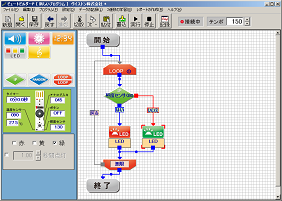
\includegraphics[width=8cm, bb=0 0 1006 770]{img/BeautoBuilderP_SSs.png}
\end{center}
\caption{ビュートビルダーの画面}
\end{figure}
また、2013年6月5日に安倍政権の経済政策「アベノミクス」の「第3の矢」として発表した成長戦略の素案には、「産業競争力の源泉となるハイレベルな IT人材の育成・確保」という項目があり、その中には「義務教育段階からのプログラミング教育等のIT教育を推進する」との記載があった[1]。今後、日本のプログラミング教育はさらに拡大していくことが予想される。

しかし、今の中学校のプログラミング教育ではソースコードを打ってプログラミングをするということを行っておらず、プログラミングの内容を深く取り上げていない。また、プログラミングを学べるのは中学校3年生の時だけで、イギリスやエストニアと比べるととても短い期間である。高校では、実際にプログラミングを教えているところもあるが、義務化さていないので誰もが学校でプログラミングを学べるわけではない[6]。
\bunseki{中進吾}

\section{現状と課題}
日本の中学校ではビジュアルプログラミング言語を用いたプログラミングの授業を行っており、ソースコードを書く練習は行っていない。ビジュアルプログラミング言語はC言語やJavaのようなプログラミング言語と表記の仕方が大きく異なっている。そのため中学校の授業だけでは、C言語やJavaのように実際に文字を打ち込むようなソースコードを組もうとした時、どのように組んでいいかわからない。Webサイトやアプリなどのシステム開発を行う際、基本は文字を打ち込むプログラミング言語を用いるので、ビジュアルプログラミング言語はほとんど使用しない。今の中学校のプログラミング教育だけでは、産業競争力の源泉となるハイレベルな IT人材の育成・確保をすることはできない。現状のままでは、イギリスやエストニアなどの他国との差が広がる一方である。
\bunseki{中進吾}

\chapter{前期のプロジェクトの目標}
\section{開発アプリの目標}
背景で述べたように、世界中でプログラミング教育の必要性が高まっており、実際に小学生からアプリ開発の授業を行っている国もある。日本でも中学校の技術家庭科でプログラミング教育が必修項目となっている。しかし、現在の中学校のプログラミング教育ではソースコードを打ってプログラミングをするということをしておらず、プログラミングの内容を深く取り上げていない。
\par
そのため、中学校でプログラミングを学んだ人、興味をもった人を対象として、中学で学んだプログラミングと実際のプログラミングの間のプロセスを支援し、ソースコードの組み立てを学ぶことが出来るゲームアプリを開発する。そこで、ビュートビルダーやScratchのようなビジュアルプログラミング言語を学んだ中学生が、C言語のように実際に文字を打ち込むようなソースコードの組み方を理解できるようになることが、開発アプリの目標である。
\bunseki{皀勢也}

\section{プロジェクト学習としての目標}
新しいプログラミング言語であるSwift言語を使い、アジャイル開発手法の一つであるScrumという方法論を用いて素早いアプリ開発をする。また、短期間での開発とフィードバックを繰り返し、より良い品質のアプリ開発を目指している。さらに、バージョン管理システムの理念を学び、効率よくアプリ開発する。プロジェクト学習を通して、情報システムコース、高度ICTコースや情報デザインコースなど異なるコースのメンバーで開発を進めていく。開発を進めていく中で、コミュニケーション能力、グループ開発力を養い、異なる分野の知識を吸収する。
\par
プロジェクト学習としての最終的な目標はアカデミックリンク、成果発表会や課外発表会でアプリの発表を行いレビューを受け、受けたレビューを反映させたアプリをリリースすることである。
\bunseki{皀勢也}

%3章
\chapter{前期の活動}

\section{プロジェクト全体としての活動}

\subsection{スクラッチワークショップへの参加}
\par 教育をテーマにするに当たり、まず小学生と触れ合い、教育の現状について考えるために、原田先生主催のワークショップに参加した。ワークショップは、2015年5月9日に、函館市青年センターにて行われ、小学校5年生から中学校1年生の子供達計10人が参加した。ワークショップの内容は、ビジュアルプログラミング言語「Scratch」を用いて、動きに反応して音が鳴る不思議楽器を作るというものである。当日、メンバーは小学生の側についてプログラミングのアシスタントをした。

\begin{figure}[H]
\begin{center}
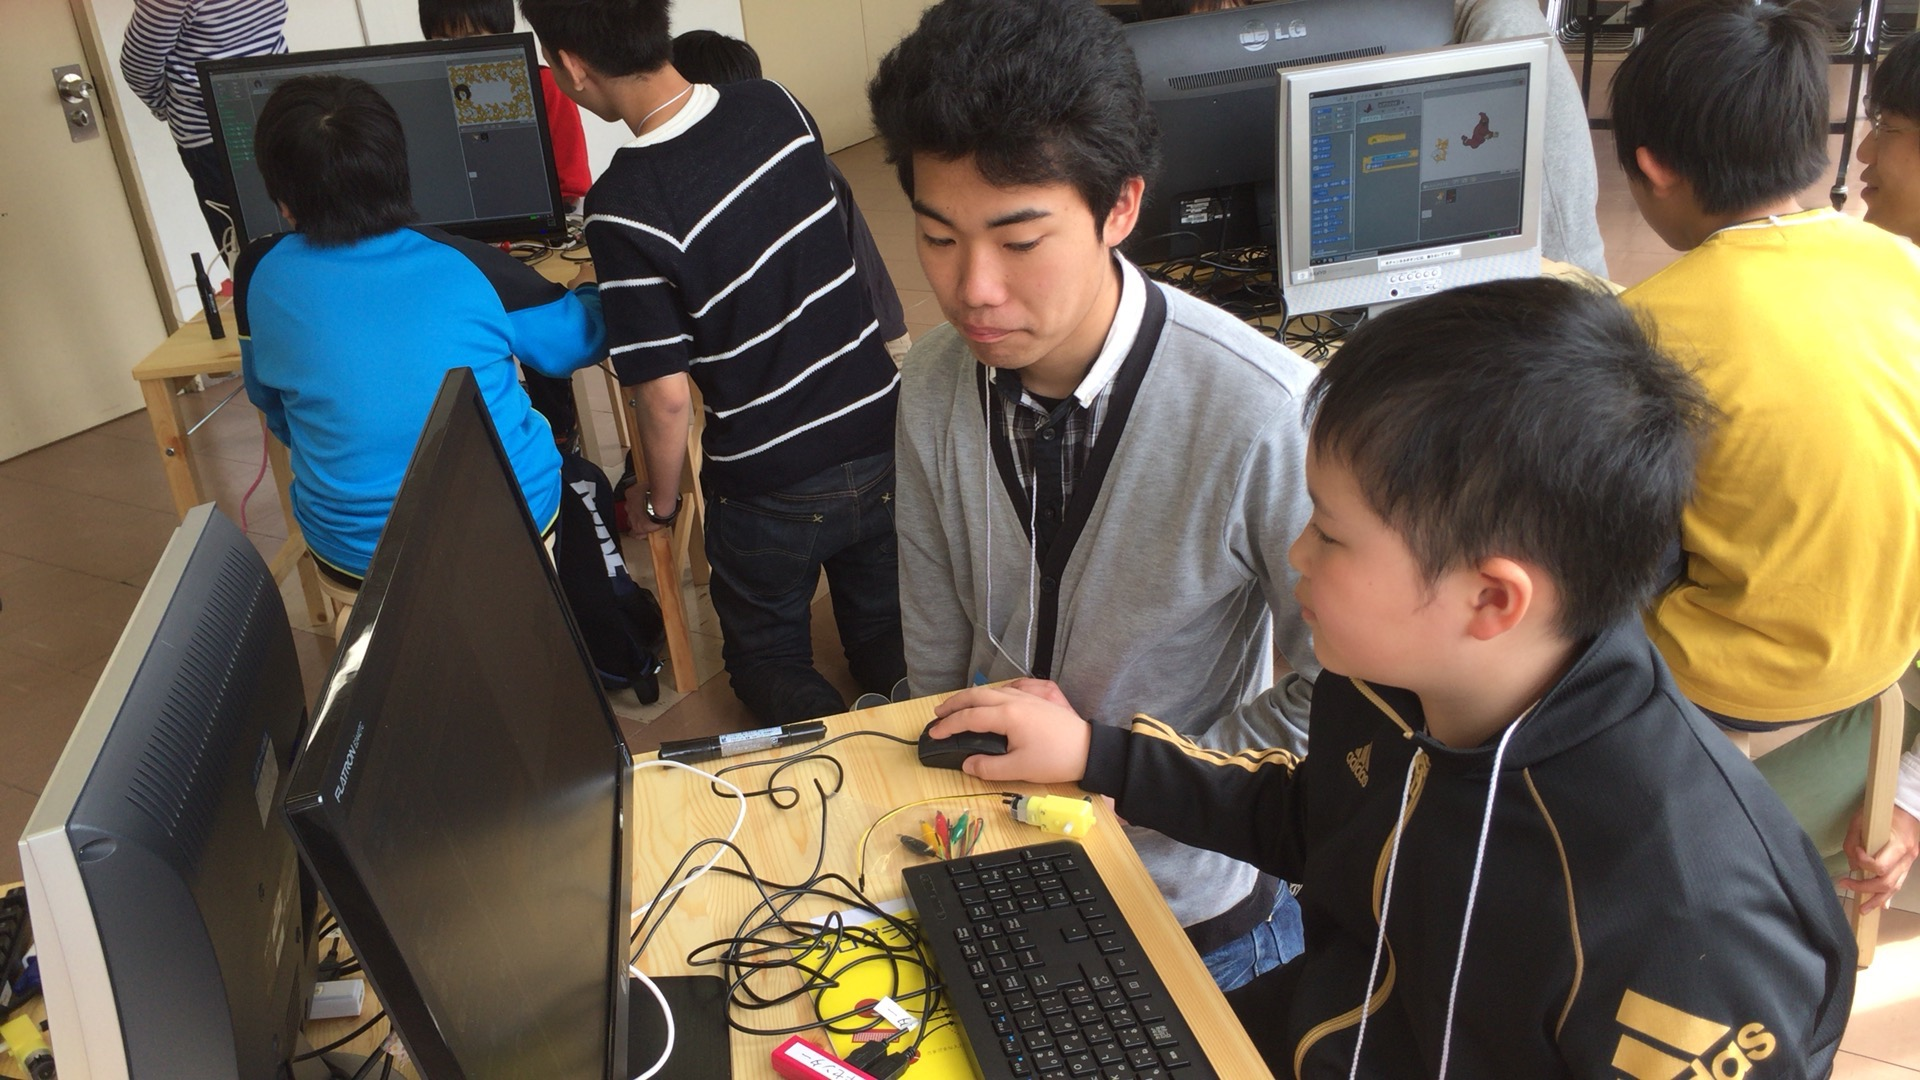
\includegraphics[width=14cm, bb=0 0 1920 1080]{img/20150509_workshop.jpg}
\end{center}
\caption{スクラッチワークショップの様子}
\end{figure}

\par ワークショップを通して、気づいた点は次の2点である。
\begin{itemize}
\item 子供達は、一度得た知識はすぐに自分のものにしているようだった。今回のワークショップは、前回のワークショップ参加者から引き続き参加している子供が多いということもあって、メンバーが使い方を教えるまでもなく、自力でプログラミングを行っていた。更に、繰り返し文の使い方を教えたところ、「じゃあさ、ここもこうすればいいんじゃない?」と、子供自ら別の点の修正を行っていた。子供の成長能力の高さに驚いた。
\item 前回から参加している子供に、どうして今回も参加したの?と尋ねたところ、「だって、これ(Scratch)楽しいんだもん」と答えた。子供でもプログラミングに興味を持っていることに驚いた。
\end{itemize}

\par また、ワークショップの最後に、参加者の子供達と、その親に向けた簡単なアンケートを実施した。しかし、プロジェクトとしての方針が決まってない状態で作成したアンケートだったため、内容が建設的なものではなく、得たアンケート結果をその後に生かすことが出来なかった。むしろ、アンケート内容に子供にはわかりづらい表現がある、難しい漢字を使っている、子供用と大人用のアンケート用紙の区別がつかないといった問題を発見できたことが、その後に生かせる学びであったと言える。

\bunseki{熊谷優斗}

\subsection{リスク分析}
\par プロジェクトを進めるにあたって起こりうるリスクをメンバーそれぞれで洗い出し、それぞれのリスクに対して発生確率、被害の内容、対処方法を挙げた。図3.2は洗い出したリスクの一部である。

\par リスクの洗い出しをした時点で既に発生していたのが、「メンバーに連絡がつながらない」というリスクだ。前述のスクラッチワークショップにてアンケートを実施したが、このアンケートを作成する際、メンバーの1人に連絡がつながらず、ワークショップ当日になってそのメンバーにアンケート内容のレビューをしてもらった結果、いくつかの不備があることが発覚した。この不備は、そのメンバーが前日にアンケート内容をレビューできていれば気づけたはずである。今後このようなリスクが発生しないよう、メンバー内で1日1回はSkypeやLINEを確認することを義務づけた。

\begin{figure}[H]
\begin{center}
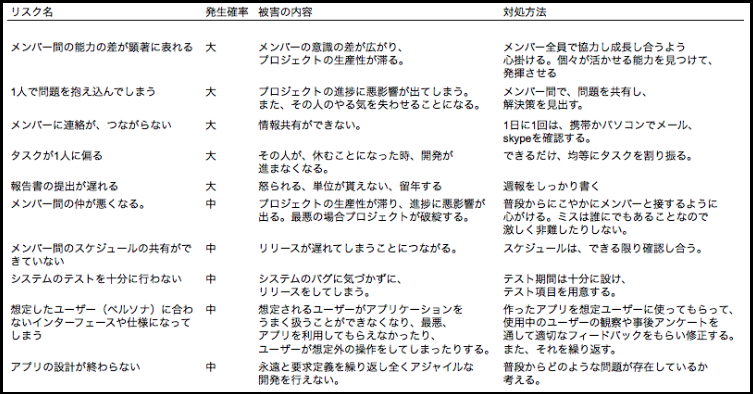
\includegraphics[width=14cm, bb=0 0 753 394]{img/RiskManagement.png}
\end{center}
\caption{リスク分析の結果(一部抜粋)}
\end{figure}

\bunseki{熊谷優斗}

\subsection{アプリ開発のための勉強会}
\par iOSアプリを開発するにあたって必要となる知識を学ぶ勉強会をプロジェクトのティーチングアシスタントが開催したため、これにグループ全員で参加した。勉強会では、XcodeやSwift言語の使い方を学ぶSwift勉強会とバージョン管理システムである、GitとGitHubの使い方を学ぶGitHub勉強会の2種類が行われた。それぞれで行ったことを具体的に記述する。
\par Swift勉強会は全部で3回行われた。第1回では、メンバーそれぞれのPCにXcodeを導入し、Swift言語によってIBLabelやIBButtonを用いた簡単なアプリを作成した。その後、iPadにて作成したアプリをビルドするために、iOS Developer Programへの登録を行った。第2回では、MapKitというFrameworkを用いた地図アプリを作成した。第3回では、サーバーからデータを読み書きすることのできるアプリを作成した。それぞれの回の終わりには演習問題が出され、これを解くことで学んだ知識の復習を行うことができた。
\par GitHub勉強会は全部で3回行われた。それぞれの回を通して、バージョン管理システムの理念を学びつつ、Gitの基本的な使い方を学んでいった。第3回では、Swift勉強の演習問題をGitHubを用いてメンバー間で分担しながら作成せよ、という課題が出た。しかし、上手くコーディングの役割分担を行うことができず、1人で全てのコーディングをし、残りのメンバーでコードレビューをするという形を取った。これに対し、ティーチングアシスタントから昨年度はもっと役割分担ができていた、という報告を受けた。今後、上手く役割分担をしていくために教育班では、GitHub の issue 機能を利用していくことを決定した。
\bunseki{熊谷優斗}

\subsection{バックログの作成}
\par プロジェクトの方針として、アジャイル開発手法の1つであるScrumという方法論を取り入れることが決まっていたため、プロジェクトのスケジュールをバックログを用いて管理した。バックログとは成果物を作り出すために必要な要素を項目に起こした一覧のことで、この一覧を上下に整頓することで項目の優先順位を表す。バックログには明確なスケジューリングをする必要はなく、優先順位の高いものから順番に行っていく。図3.3は6、7月分のバックログの原案である。はじめに設計を行っていくことをしたかったため、「画面遷移図を作成」や「マップ画面設計」といった、設計に関するタスクの優先順位を高くした。

\par この原案を企業講師である高森満様と木下実様にお見せしたところ、「バックログの優先度を議論する際にもっと手軽に入れ替えることが可能なように、紙や付箋を用いたほうが良い」というレビューを受けた。そこで、せっかく紙と付箋を使用するならばと、ソフトウェア開発のツールの1つである、「タスクかんばん」のシステムをバックログに取り入れることにした。図3.4は実際に使用しているバックログである。図のように、タスクの状態を「TODO」、「DOING」、「DONE」の3つのステージに分割し、更に「TODO」欄のタスクの上下関係によってタスクの優先度を表すようにした。

\begin{figure}[H]
\begin{center}
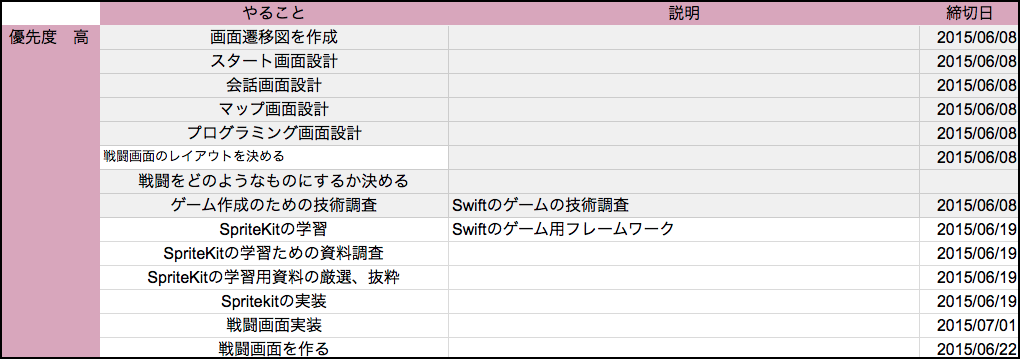
\includegraphics[width=14cm, bb=0 0 1020 359]{img/SprintBacklog.png}
\end{center}
\caption{6、7月分のバックログの原案}
\end{figure}

\begin{figure}[H]
\begin{center}
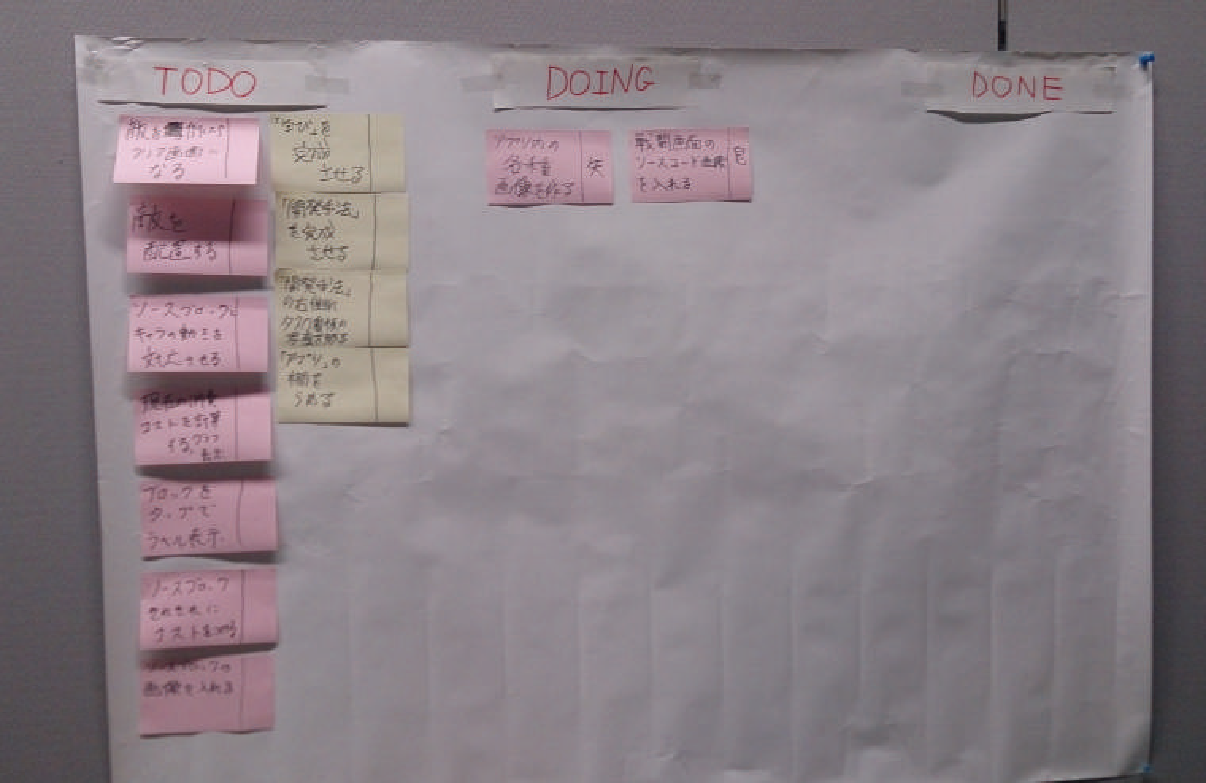
\includegraphics[width=14cm, bb=0 0 1206 783]{img/TaskKanban.png}
\end{center}
\caption{タスクかんばんのシステムを取り入れたバックログ}
\end{figure}

\bunseki{熊谷優斗}

\subsection{中間発表会の資料制作}
\par 中間発表会に向けて、ポスターを制作した。制作にあたって、グループメンバーを実装班3人とポスター班2人に分け、ポスターの制作が終わったら実装班がレビューをする、という形式をとった。しかし、メンバー間の意識共有が上手く行われていなかったため、実装班がポスターのレビューを上手く行うことが出来なかった。そのため、ポスターをティーチングアシスタントや担当教員に見せたところ、目的と制作物がずれている、というレビューを受けた。これを受けて、メンバー5人全員で、一度背景、目的、課題の見直しを行い、ポスターの作り直しをした。しかし、短期間で急いでポスターの作り直しを行ったため、今度は文字が多すぎて見づらいというレビューを受けた。これを受けて、ポスター内の文字を少なくするため、もう一度ポスターの構成を見直すという作業を行った。結果、ポスターを作り上げることができたが、その制作に多くの時間を割くことになってしまった。ポスターやその他ドキュメントを作る際には、まずメンバー間の意識共有を行い、どういった構成で文書を書いていくのかを考えることに時間をかけるべきだ、ということを学んだ。

\bunseki{熊谷優斗}

\subsection{中間発表会}
\par 中間発表会ではメンバーを前半3人、後半2人に分けて、発表を行った。前半の発表では、アプリのデモを行わないと内容が伝わりづらい、というレビューを受けた。これを受けて後半の発表では、デモを取り入れ、内容が伝わりやすいようにした。しかし、後半の発表では合計で9人しか見に来た人がいなかった。このことから、教育系が開発しているアプリに魅力が少ないのではないか、という気づきを得た。

\bunseki{熊谷優斗}

\section{アプリ案の変化と内容}
\par プロジェクトを進めるうちに、アプリ内容、対象ユーザーが変化していった。図3.5にその流れを示す。

\begin{figure}[H]
\begin{center}
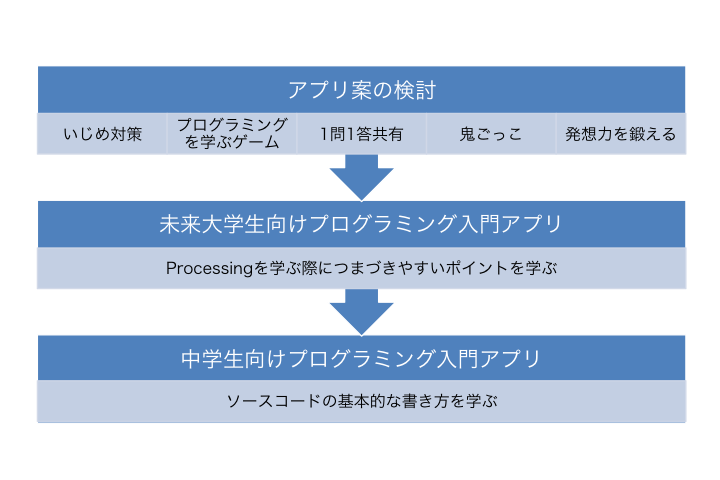
\includegraphics[width=12cm, bb=0 0 720 480]{img/appChangeFirstTerm.png}
\end{center}
\caption{アプリ案の変化}
\end{figure}

\bunseki{熊谷優斗}

\subsection{アプリ案の検討}
\par メンバーそれぞれが考えて来た案を評価し、5種類の案に絞った。図3.6に案を表す。

\par 5種類それぞれの案をメンバー内で肉付けした後、ティーチングアシスタントと担当教員からレビューを受けた。それぞれの案の詳細とレビューの内容を以下に示す。

\begin{description}
 \item[案1 いじめ対策アプリ]
従来相談を受けてもらうためには、電話をかけ、言葉で喋らなければならないので、ハードルが高い。一部の教育委員会では、メールの対応も行っている。そこで、少しでもハードルを下げるために、LINEのように教育委員会と会話ができるようにする。
\begin{description}
 	\item[レビュー内容]

	このままだとただチャットをするだけのアプリになってしまうのではないか。既存のSNSアプリと差別化を行うため、独自の機能が必要である。また、どのようにしてこのアプリの評価を行うかという点は要検討である。
	 \end{description}
 
  \item[案2 プログラミングを学ぶゲームアプリ]
子供がゲーム攻略を楽しみながら、いつのまにかプログラミングを覚えることができるアプリである。最終的なユーザーの到達点としては制御文が使えるようになることである。
	\begin{description}
 	\item[レビュー内容]
	ゲーム内容は、答えを導くのに手間がかかり、ユーザーに達成感があるものにすべきである。似たようなアプリは既にいくつも存在しているため、それらを調査し、どのように差別化を図るか検討する必要がある。
	 \end{description}

  \item[案3 発想力を鍛える−生産消費的なゲームアプリ]
  ユーザーが生産側と消費側の両面で機能することにより、全ユーザーで一緒に発想力を磨いていくアプリである。自分よがりの発想力ではなく、他人にも共感できる発想力を身につけさせることが目的である。
	\begin{description}
 	\item[レビュー内容]
	ユーザー依存型アプリは投稿が増えないと開発が進まない可能性があるため、どうしたらユーザー同士で活発に活動してもらえるか考えるべきである。
	 \end{description}
	 
 \item[案4 1問1答共有アプリ]
  ユーザーが作った1問1答を共有するアプリである。問題を作る楽しさと問題を解く楽しさをシェアすることができる。
	\begin{description}
 	\item[レビュー内容]
	案3と同様に、どうしたらユーザー同士で活発に活動してもらえるか考える必要がある。投稿者が何か得をするシステムにしなければ問題の投稿数は増えていかないだろう。
	 \end{description}
	 
 \item[案5 外遊び支援アプリ]
遊びの教育を行う。IT化が進み、外で遊ぶことが少なくなってきている子供たちに対し、ITを活用することで子供に外で遊んでもらう機会を増やす。その1つの案として、GPS機能を使って鬼ごっこを行う。
	\begin{description}
 	\item[レビュー内容]
	このアプリを開発するのであれば、楽しく開発を行えるだろう。しかし開発者が楽しくてもユーザーが楽しいとは限らない。ユーザーがどのような遊びを求めているか調査する必要があるだろう。また、アプリを使いながら鬼ごっこをすると、歩きスマホのような状態になり危険なのではないか。
	 \end{description}

 \end{description}
 
 \par レビューを受け、グループ内で検討した結果、前期では「案2 プログラミングを学ぶゲーム」を作成することに決定した。
 
 \begin{figure}[H]
\begin{center}
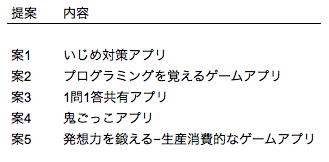
\includegraphics[width=12cm, bb=0 0 329 162]{img/AppIdea.png}
\end{center}
\caption{絞った5種類のアプリ案}
\end{figure}
 
 \bunseki{熊谷優斗}
 
 \subsection{大学生向けプログラミング入門アプリ}
\par 前述の「案2 プログラミングを学ぶゲーム」についてより深く考えていった結果、「既存の類似アプリと相違点を持たせるため、函館要素を追加しよう」、「子供は地域性に対してあまり興味を示さない、ならば対象ユーザーを未来大生にしよう」といった理由から、未来大学に入学することが決まった高校生に対するProcessing導入アプリを作成する方針が決まった。アプリの目的は、未来大1年生が「情報表現入門」でプログラミング言語「Processing」を学ぶ際につまづきやすいポイントを、入学前にゲーム形式で気軽に学んでもらうことである。図3.7と図3.8はアプリ内画面のイメージ図の一部である。

\par 図3.8、通称「プログラミング画面」では、Scratchのように主人公の行動を表すブロックを組み立ててゆく。どのようなブロックを組めばいいかを考え、それにより主人公を操り、敵を全て倒すことがゲームの目的である。更に、「コスト」という概念を定義し、ブロックそれぞれをコストで重み付ける。1ターンで使用できるコストの上限は決まっているので、ユーザーはどのようにブロックを組めば同じコストでも最も多く行動できるかを考える必要がある。例えば、ループ文を使うことで、単純に同じブロックを何度も使用するよりも少ないコストで済む。これによりユーザーは自然と良いアルゴリズムを学ぶことができる。
\par このアプリ案をティーチングアシスタント、担当教員、企業講師の方々に見せたところ、様々なレビューを受けた。一部を抜粋すると次のようなものである。
\begin{itemize}
 \item このアプリをプレイしたところで、本当にプログラミングの教育になるのだろうか。肝心のプログラミング画面の内容が薄く、未来大生がつまづきやすいポイントを学べるとは思えない。どうすればユーザーへの「教育」になるかを練り直すべき。
 \item 大学生が使うにしては、プログラミング画面の内容が低年齢向けである。
 \item もしアプリを一般向けにリリースすることを目標としているのであれば、未来大学入学向けアプリというのは対象ユーザーが狭すぎる。
 \end{itemize}
\par このレビューを受けて、もう一度メンバー内で教育要素について考え直し、対象ユーザーを全国の高校生、大学生向けへと変更した。また、プログラミング画面にて、「→」「パンチ」といった簡単な記述ではなく、「move(right, 3)」「attack(up)」といった、より本物のソースコードに近い形で表示するようにし、そのソースコードはボタンをタップしていくことで組み立てることができる仕組みにした。

\begin{figure}[H]
\begin{center}
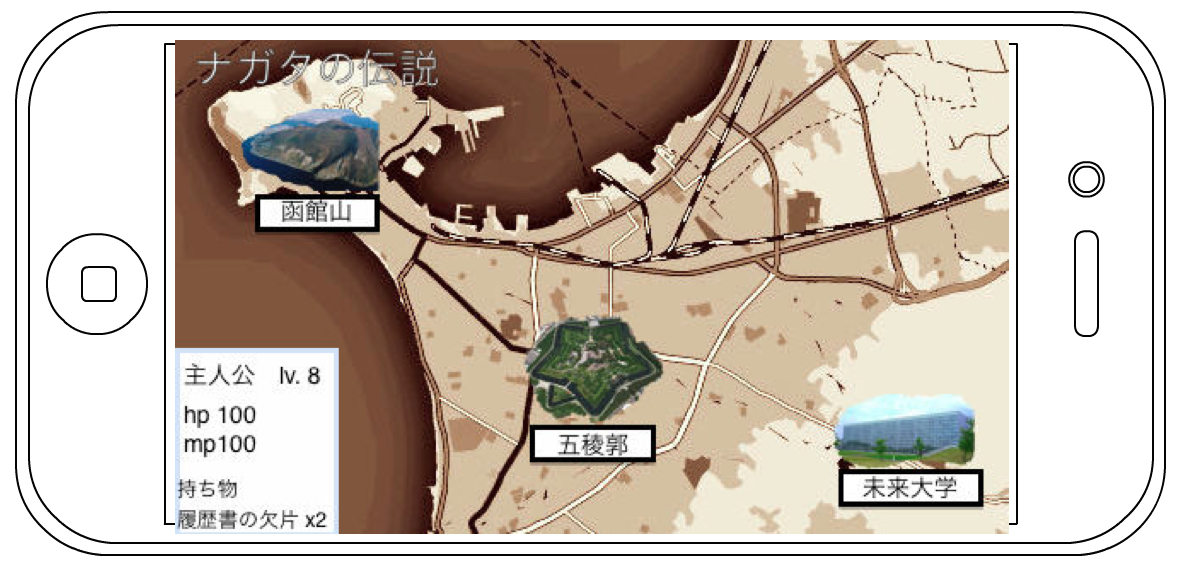
\includegraphics[width=12cm, bb=0 0 1182 571]{img/LengedOfN_map.png}
\end{center}
\caption{マップ画面}
\end{figure}

\begin{figure}[H]
\begin{center}
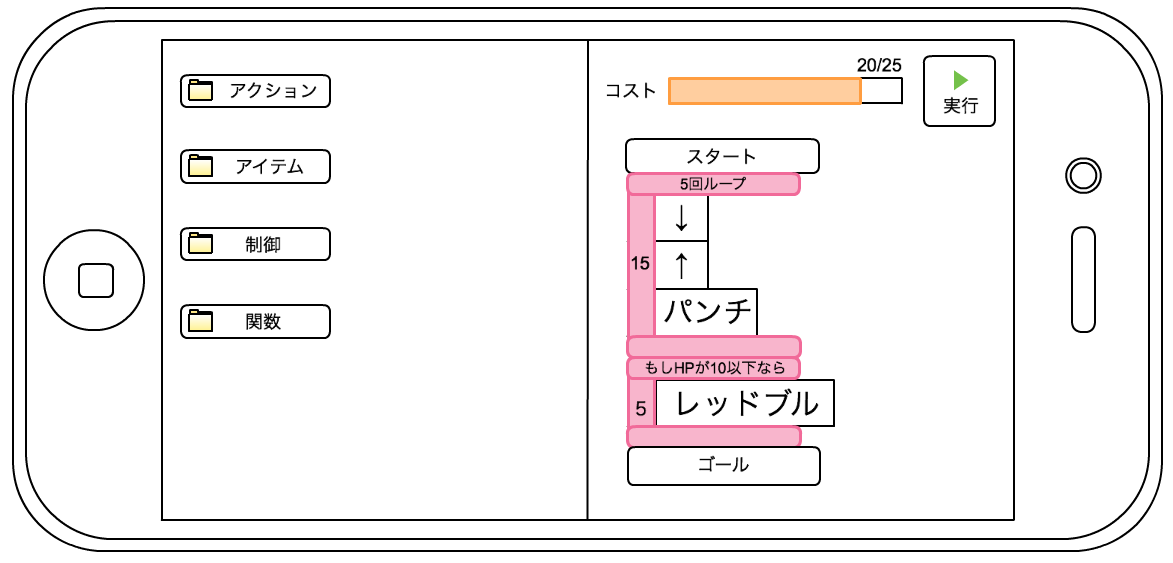
\includegraphics[width=12cm, bb=0 0 1173 563]{img/LegendOfN_programming.png}
\end{center}
\caption{プログラミング画面}
\end{figure}
 \bunseki{熊谷優斗}
 
 \subsection{中学生向けプログラミング支援アプリ}
\par プロジェクトを進めるうちに、大学生向けプログラミング入門アプリでは、プロジェクトとしての背景が、客観的に見て共感されないような内容であることに気がついた。そこで、日本の中学校ではプログラミング教育が義務化されている、また、現状のアプリ内容であれば、小学生、中学生が利用しても問題がないといった理由から、対象ユーザーを変更すべきであるという結論にたどり着いた。この日の議論により生まれたのが現状の背景(第1章にて記載)であり、現状のアプリ案(第4章にて記載)である。

\bunseki{熊谷優斗}

%4章
%%%%%%%%%%%%%%%%%%%%%%%%%%%%%%%%%%%%%%%%%%%%%%%%%%%

\chapter{前期の開発アプリについて}
\section{概要}
開発するアプリは中学生でプログラミングを習った人、興味を持った人を対象としたソースコードの組み方を学ぶゲームアプリである。図4.1のように、このゲームには自機と敵機があり、ユーザーはマス目上のステージにある自機をソースコードを組むことによって動かし、敵機を倒すことでゲームがクリアとなる。

%\\
\begin{itemize}
\item 各ステージのクリアまでの流れ
\end{itemize}
\begin{enumerate}
\item 自機を敵機の前まで移動して倒すソースコードを考える。
\item ソースコードを入力する。
\item ソースコードを実行する。
\item ソースコードの通りに自機が動く。
\item 敵を全て倒すとステージクリアとなる。
\item 使用したコストに合わせてランクとコメントが表示される。
\end{enumerate}
\par 敵機まで移動して倒すまでをいかに短いソースコードで完了させるかを目指すゲームである。

\begin{figure}[h]
\begin{center}
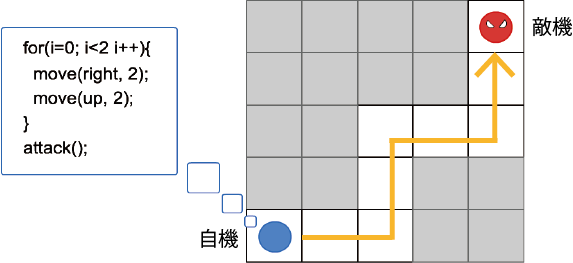
\includegraphics[width=12cm, bb=0 0 573 263]{img/4thParagraph/game.png}
\end{center}
\caption{ゲーム概要}
\end{figure}

\bunseki{新保遥平}

\section{プログラミング画面}
プログラミング画面ではユーザーが敵機を倒すためのソースコードを入力する。例えばfor文を入力したいときは図4.2のように画面に配置されたソースボタンをタップする。

\begin{figure}[H]
\begin{center}
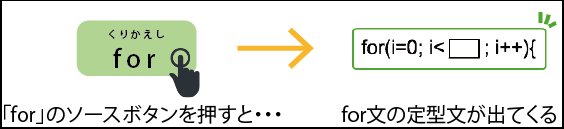
\includegraphics[width=12cm, bb=0 0 564 129]{img/4thParagraph/forButton.png}
\end{center}
\caption{ソースコードの入力}
\end{figure}
ユーザーは図4.3のように画面右側に配置されたそれぞれのソースボタンをタップして、ソースコードを組み立てていく。現状、実装したソースボタンはattack()、move()、left、right、0〜9、;  などである。タップされたソースボタンは順に、右側のスペースに記述される。


\begin{figure}[H]
\begin{center}
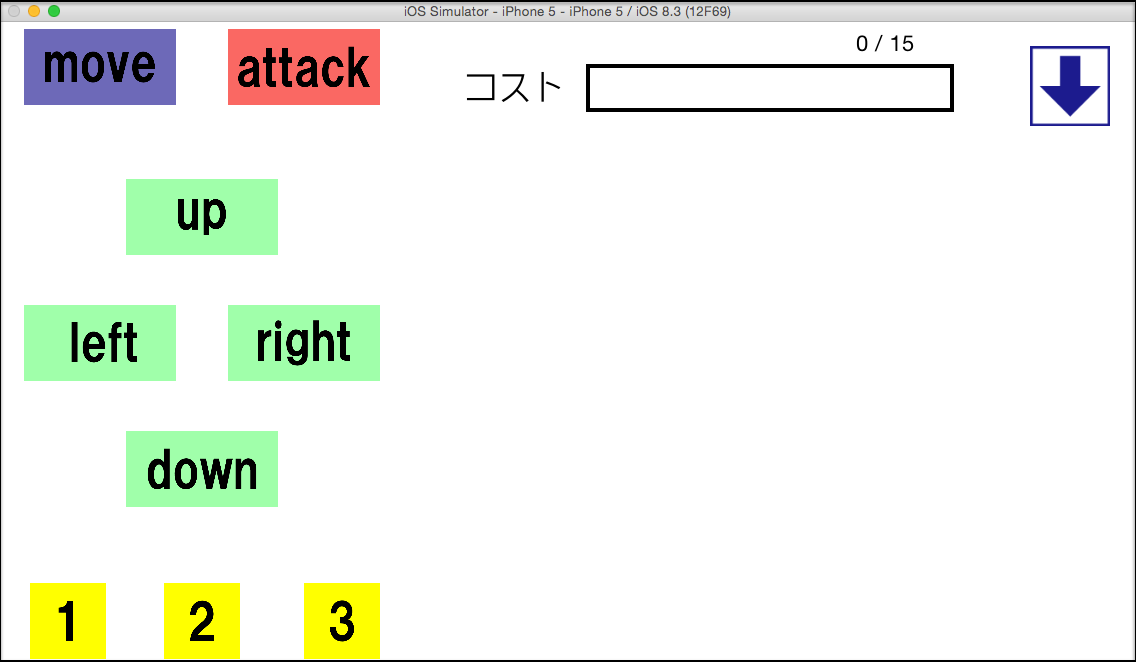
\includegraphics[width=12cm, bb=0 0 1136 662]{img/4thParagraph/Prog-ra_programming.png}
\end{center}
\caption{プログラミング画面}
\end{figure}

例えば下記のようなプログラムを組むこととする。
\par move(right,3);
\par move(up,3);
\\
\\
このソースコードを図4.4のプログラミング画面に入力した。

\begin{figure}[H]
\begin{center}
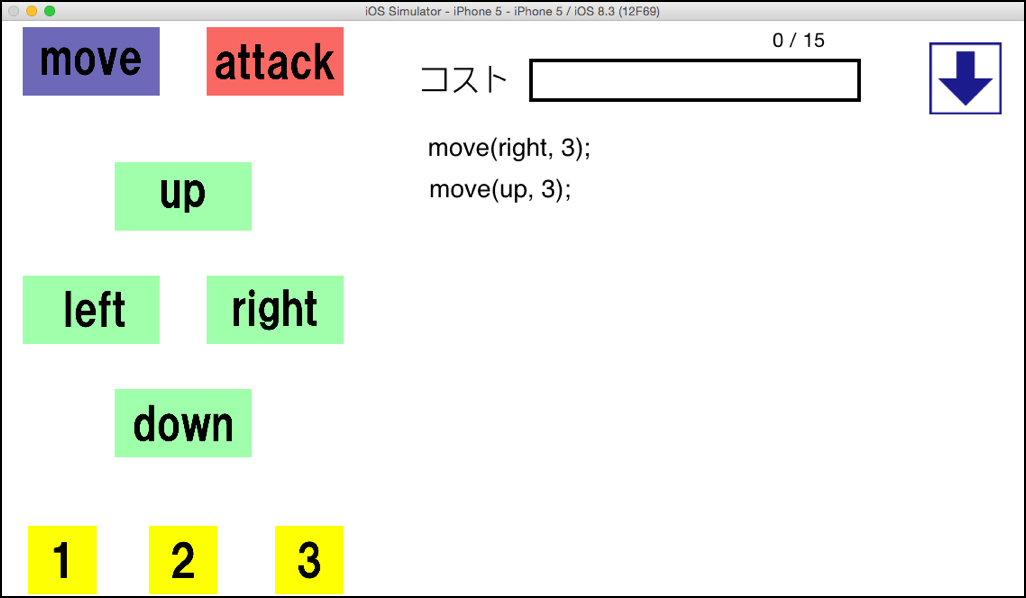
\includegraphics[width=12cm, bb=0 0 1136 662]{img/4thParagraph/Prog-ra_programming1.png}
\end{center}
\caption{ソースコード入力後のプログラミング画面}
\end{figure}

このようにプログラムをタップで組むことが出来る。また、図4.5のようのに、次に引数である数字を入れるべきところに「up」をタップしてしまうなど、間違ったタイミングでソースボタンを押すと画面上にエラーが出て、すぐに確認ができる。


\begin{figure}[H]
\begin{center}
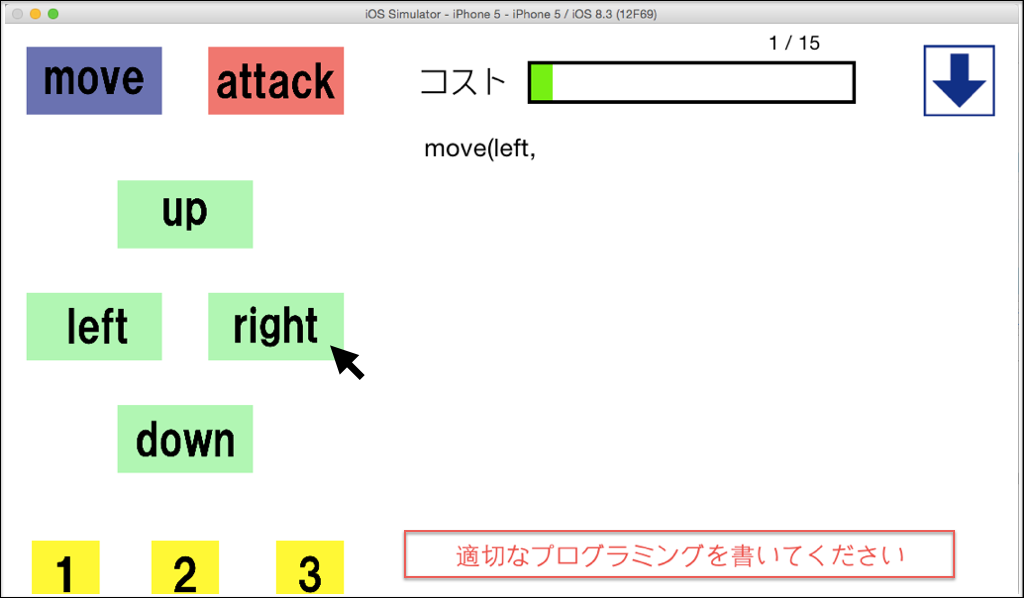
\includegraphics[width=12cm, bb=0 0 1024 598]{img/4thParagraph/error.png}
\end{center}
\caption{ソースコードがエラー時のプログラミング画面}
\end{figure}
ユーザーはソースコードを入力後、プログラミング画面の左上の「下矢印」ボタンで戦闘画面に移動する。

\bunseki{新保遥平}

\section{戦闘画面}
図4.6の戦闘画面はプログラミング画面で入力したソースコードで自機を動かすための画面である。戦闘画面の左下にある三角の実行ボタンを押すことで、自機を動かすことが出来る。また戦闘画面、左下の「P」と書かれたボタンでプログラミング画面に戻ることができる。現状では、あらかじめ設定されたプログラムでしか自機を動かすことが出来ない。

\begin{figure}[H]
\begin{center}
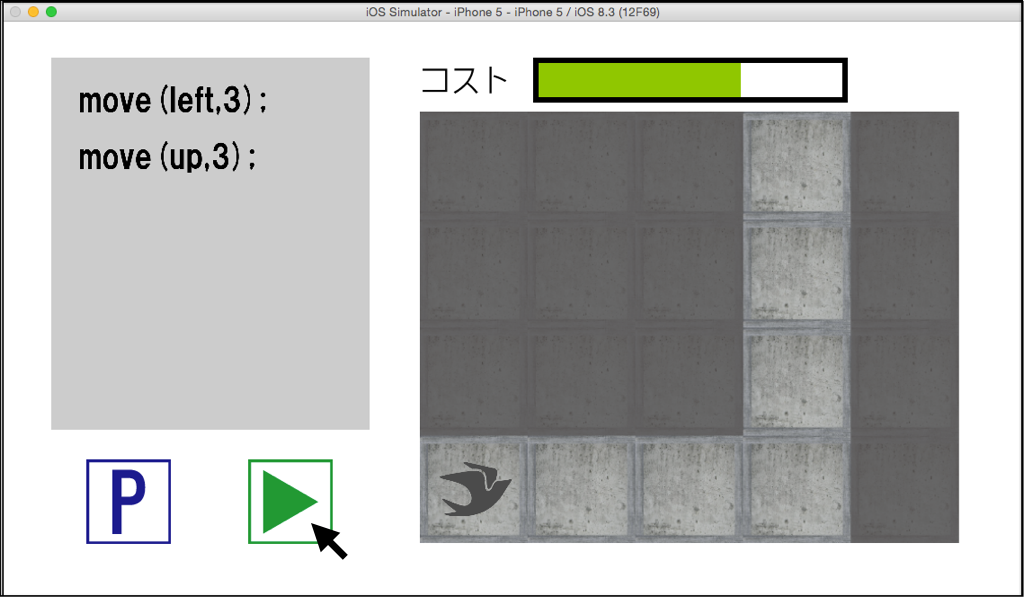
\includegraphics[width=12cm, bb=0 0 1136 662]{img/4thParagraph/Prog-ra_Battle.png}
\end{center}
\caption{戦闘画面}
\end{figure}

\bunseki{新保遥平}

\subsection{ゲーム性}
ただプログラミングを学ぶのではなく、ゲームを通してプログラミングを学ぶことでユーザーのモチベーションを保ちつつ、アプリを使ってもらえると考えた。また実際にソースコードを組むことで自機を思い通りに動かすことが出来たときにプログラミングの学習が深まると考えた。
 
\bunseki{新保遥平}


\subsection{教育性}
このアプリではユーザーがより簡潔なソースコードを組み立てられるようになるために、コストとランクがある。ソースのボタンそれぞれにコストが設けられており、問題をクリアした際にコストの使用量が少ないほど簡潔にソースコードを組み立てることが出来たと判定し、図4.7のようにランクを与える。ランクが低かった場合、より良いランクにつながるヒントを与える。そして高いランクが与えられたときに、ユーザーを褒める言葉を表示する。このサイクルが次の問題への意欲につながり、より簡潔なソースコードを組み立てることが出来るようになる。この流れをユーザーストーリーとしたものを図4.8に示す。

\begin{figure}[H]
\begin{center}
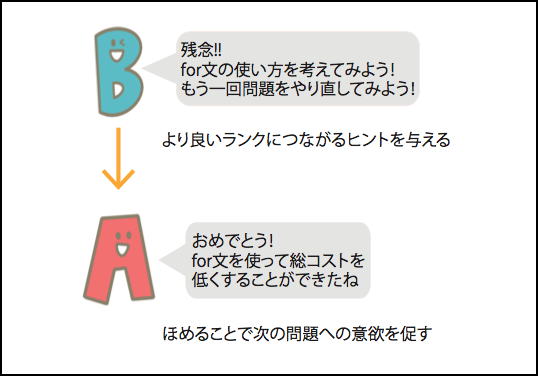
\includegraphics[width=12cm, bb=0 0 538 376]{img/4thParagraph/cost.png}
\end{center}
\caption{ランクとヒント}
\end{figure}

\begin{figure}[H]
\begin{center}
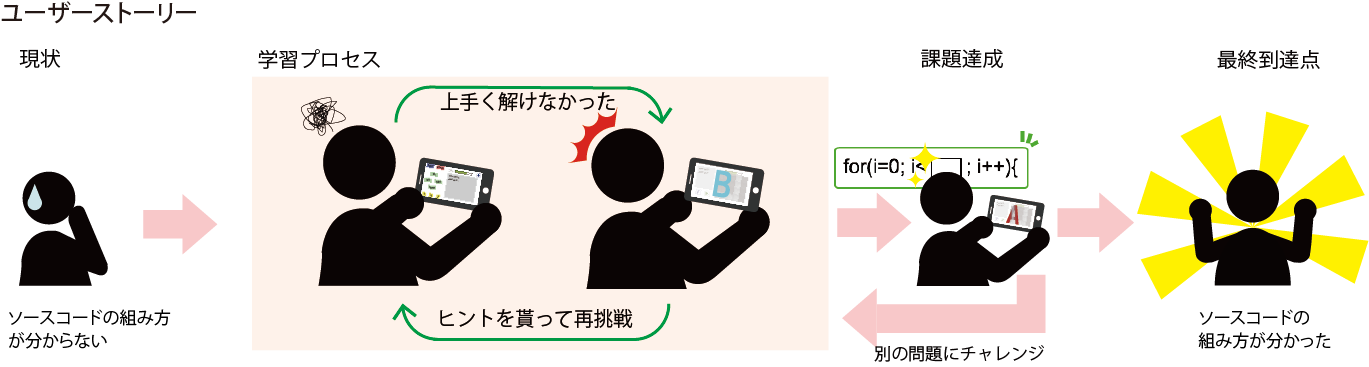
\includegraphics[width=14.5cm, bb=0 0 564 129]{img/4thParagraph/userstory.png}
\end{center}
\caption{ユーザーストーリー}
\end{figure}







\bunseki{新保遥平}
%%%%%%%%%%%%%%%%%%%%%%%%%%%%%%%%%%%%%%%%%%%%%%%%%%%

%5章
\chapter{前期の結果}
\section{プロジェクトの評価}
本プロジェクトは、多くの方からレビューを受け今の背景、課題、目的になっている。しかし、私たちが考えたアプリはその課題を解決できるアプリとなっていない。そのため、アプリの設計を見直す必要がある。

また、7月に行われた中間発表会の評価シートの結果からは、「声がはっきり聞こえた」、「声は大きく聞きやすかった」、「相手の顔を見て話してくれたので、聞き取りやすかった」などの意見をいただき、発表技術に関しては高い評価を得られた。しかし、発表内容に関しては「最終的なゴールは?」、「内容がわからないないので評価不能」、「既存のもとの比較がない」などの意見をいただいた。いただいた意見をまとめると、本プロジェクトは目標が決まっておらず、内容がわかりづらいという評価であった。

これらのことから、本プロジェクトは第三者の方に伝えられる内容になっていないので背景、課題、目的につながるアプリ案が必要である。そして、第三者の方に伝えられる内容にしていかなければならない。
\bunseki{中進吾}

\section{プロジェクトの成果}
\par 前期の活動の成果は以下の3点である。
\begin{itemize}
\item スクラッチワークショップに参加したことにより、プログラミング初心者の方にプログラミングを教える場合、C言語やJavaから始めるのではなく、Scratchのようなビジュアルプログラミング言語から始めた方が良いということがわかった。また、プログラミングで音声機器などの機械を動かしてもらうことにより、プログラミングに興味を持ってもらうことができるということがわかった。
\item 
本プロジェクトでは、Swift言語を用いてアプリ実装を行うことになっていた。しかし、メンバー全員Swift言語は使ったことがなかったため、実装に不安があった。アプリを実装できる期間は短かったが、キャラクターを動かしたり、ボタンをタップすることでソースコードを打ち込めることができるところまでアプリを開発することができた。これによって、今後のアプリの実装に対する不安がほとんどなくなった。また、アプリの実装を行えたことにより、実装に携わったメンバーはSwift言語に自信を持つことができた。

\item 中間発表会で展示するポスターは、Adobe Illustratorという描画ツールソフトを使用して作成することになっていた。このソフトを使用したことがあるのはメンバーの5人中2人だけだったため、ポスターを作成できるのは2人だけだった。しかし、3.1.5で述べたように目的と制作物がずれていたため、メンバー 5人全員で、一度 背景、目的、課題の見直しを行い、ポスターを作り直すことになった。その結果、今までAdobe Illustratorを使ったことがない人も使えるようになり、メンバー全員がポスターを作成できるようになった。11月に開催されるアカデミックリンクや最終成果発表でもポスターを使用するので、メンバー全員がポスターを作成できるようになったことは、非常に大きな成果である。
\end{itemize}

\bunseki{中進吾}


%6章
%%%%%%%%%%%%%%%%%%%%%%%%%%%%%%%%%%%%%%%%%%%%%%%%%%%

\chapter{後期の背景}

\section{プログラミング基礎の現状}
\par 公立はこだて未来大学には、学部1年生が後期に必修科目として履修する「プログラミング基礎」という講義がある。この講義は、1年生が前期に履修した「情報表現入門」で学んだことをもとに、C言語について学び、プログラミング(概念、考え方)への理解を深めることを目的としている。講義内容はプログラミング基礎概念である、変数、配列、条件分岐、繰り返し、関数、文字列、構造体などについて学ぶ内容となっている。また、講義だけでなく、演習として課題(プログラム)に取り組むことになっており、毎回の講義で課題を提出することになっている。成績の評価方法は、期末試験の結果を重視し、各回の課題の提出状況で評価されることになっている。しかし、例年「プログラミング基礎」の落第者は多くいる。「プログラミング基礎」は必修科目であるため、卒業するためには必ず単位を取らなければいけない講義である。
\bunseki{中進吾}

\section{現状と課題}
\par 私たちは、例年「プログラミング基礎」でなぜ多くの学生が落第するのか知るために、現在履修している学生とその講義を担当しているTA(Teaching Assistant)にヒアリング調査を行った。
\par 履修している学生に講義の難しい点を聞いてみると、配列などの基本的な構文が分からないということが分かった。実際に、講義で出題された課題を取り組んでいる所を見せてもらうと、講義で覚えたことをそのまま書いており、そのコードがどのように動いているのか分かっていないことが分かった。一方、TAに講義のどのような点が分からないのか聞いてみると、課題で出題される問題に対するアルゴリズムが分かっていないことが分かった。
\par 実際に講義で使われている資料を見ると、ほとんどが文字で構成されており、専門用語が多くあった。講義を履修する学生は、プログラミングを学んで日が浅い人が多いのでより分かりやすい表現が必要であると感じた。
\bunseki{中進吾}


%7章
%%%%%%%%%%%%%%%%%%%%%%%%%%%%%%%%%%%%%%%%%%%%%%%%%%%

\chapter{後期のプロジェクトの目標}

\section{開発アプリの目標}
本学の1年生が履修する「プログラミング基礎」は、C言語を学ぶ必修の講義でありながら、例年多くの1年生が落第しているという課題がある。また、1年生に対してのヒアリング調査から配列などの基本的な書き方やアルゴリズムがわかっていないことが分かった。

\par
そのため、後期の開発アプリでは、C言語やアルゴリズムを理解できていない学生に対して、講義で教える学習単元ごとに概念の説明、例題、確認問題をアニメーションで教えるWebアプリケーションを作成した。このアプリケーションを実際の授業で用い、1年生に予習、復習用の教材として利用してもらう。そこで、アニメーションを用いることで、ユーザーが学習単元の概念を理解し、実際のソースコードのアルゴリズムの動きを把握できるようになることが後期の開発アプリの目標である。
\par
後期のプロジェクトの活動で、ユーザーが適切なアルゴリズムを学べる機能を備える必要がある。迅速にプロトタイプを作成し、より多くの1年生にプロトタイプの評価を行ってもらい開発アプリをより良いものにしていく。また、概念の説明、例題、確認問題のアニメーションを完成させ、Webアプリケーションとしての体裁を整え、本大学のHOPEに掲載することを目標に活動していく。
\bunseki{皀勢也}

\section{プロジェクト学習としての目標}
前期の提案内容では、目的と提案が噛み合っていなかったため、教育性が欠けている一貫性のない提案になってしまった。また要件定義を深く行っていなく、設計を先に進めたため、目的を見失ってしまった。さらに、提案内容に関する事前調査が不十分であったため、提案内容に酷似したiOSアプリが存在していた。そのため、プロジェクトの活動を要件定義・企画の段階へと戻すことになった。
\par
後期の活動ではこれらの失敗を学び、前期のように後戻りが頻繁に起きないようにする。また、前期で行ってきた活動の経験から、グループメンバーの得意分野を活かし、メンバーの適切な役割分担を行う。さらに、本グループではICT演習に参加しているメンバーと情報デザインコースに所属しているメンバーがいるため、前期では要件定義プロセスの進め方の考えに相違があり、話し合いに時間をかけすぎてしまい、作業の遅れが生じた。後期では、双方のプロセスを学び、適切にプロジェクトを進められるようにすることが目標である。
\bunseki{皀勢也}


%8章
%%%%%%%%%%%%%%%%%%%%%%%%%%%%%%%%%%%%%%%%%%%%%%%%%%%

\chapter{後期の活動}


\section{イベント}

\subsection{後期のキックオフ}

\subsection{アカデミックリンク}
2015年11月14日に「HAKODATEアカデミックリンク2015」という函館市内などの教育機関による
合同研究発表会が行われた。このアカデミックリンクには未来大の多くのプロジェクトが参加しており、我々のプロジェクトも参加した。教育系グループはC-mationのデモとポスターをお客さん
に見せながらポスターセッションを行った。このアカデミックリンクには様々な年齢層の方がいらっしゃり、我々のアプリについて多くの意見をいただくことができた。高校生からは「こんなアプリあったらやってみたい!」、プログラミングの経験者からは「このアプリは誰かに実際に使って評価を得ることができたの?」、「本当にC言語でつまづく部分は配列なの?」などの厳しい意見を得ることができた。このアカデミックリンクではアプリの評価だけでなく、自分たちの発表する力を試すこともできたと思われる。4月にプロジェクト学習が始まって以来、何度も発表の機会があったため、メンバーの発表技術が上がり、アカデミックリンクの発表に関しては成功した。
\bunseki{新保遥平}

\subsection{最終成果発表会}


\section{アプリ案の推移}

\subsection{夏休みの課題と調査報告}
この章では、プロジェクト学習中間発表会及び中間報告書提出以降の活動から、夏休み明け序盤の活動までの経緯を示す。この期間の主な活動内容は、二点ある。一つ目は、プロジェクト学習中間発表会の反省を踏まえて、一度提案を企画立案段階まで戻し、夏休みに調査・情報収集行ったことと、もう一つは、その夏休みの活動を経て再度方向性を確立することだ。

まず、プロジェクト学習中間発表会の反省を踏まえて、一度提案を企画立案段階まで戻し、夏休みに調査・情報収集を行った活動から見ていく。私たちは前章でも述べた通り、プログラミングをするにあたって必要不可欠なアルゴリズムを、パズルゲームを通して学ぶことができるiOSアプリケーション、「プログーラ」を開発した。しかし、このアプリケーションにはいくつかの問題があり、特に以下の三つが重大な問題となった。

一つ目は、目的と提案が噛み合っていないという問題だ。これは、目的が中学校でプログラミングを習った人及び興味を持った人を対象に、プログラムの書き方を学ぶことができるゲームアプリを開発することであった。しかしながら、最終的に出来上がった提案はプログラミング要素が薄く、本当にプログラミングを学ぶことができるのかというか疑わしい結果となってしまった。

二つ目は、提案物に対する調査を深く行っていなかったという問題だ。これは、提案したゲームに酷似したiOSアプリケーションがあることが後からわかり、教育ゲームと内容及びゲーム性が被っていることから新規性にかけてしまったことだ。

三つ目は、企画立案や要件定義にあまり時間をかけずに、設計工程に入ってしまった問題だ。この原因となった最大の理由として、アジャイル開発のスクラムのやり方を勘違いしていたことがあげられる。この開発手法は簡単に言えば、迅速果断にPDCAサイクルを回していくことにことで開発していく手法だ。しかし、この手法を早くサイクルを回すことに意識が集中してしまったため、企画立案や要件定義の段階が不十分にもかかわらず、設計工程に入るという早とちりを起こしてしまった。これが引き金となり、設計工程でいつの間にか提案物のセオリーを見失い、さらには実装がスタートしてから背景情報を模索するという算段になってしまった。この問題点は、上記の二つの問題にも関わる点があり、最終的な提案物が一貫性にかけるものになってしまったことだ。

\bunseki{矢吹渓悟}

\subsection{テーマの再検討}
夏休み明けにもう一度メンバー全員で集まり、テーマの再検討を行った。そこで、前期のテーマであったプログラミング教育から離れ、観光教育が提案された。観光教育は函館国際観光コンベンション協会が函館市内の小学校で開いている「『函館観光』子ども学習会」の現状の問題をITを使って解決し、地元の魅力を地元の子供たちに伝えることである。また、自然体験のない青少年の割合が増加、子供の読書離れ、子供の体力低下、朝食離れや身近な伝統文化や現代の文化芸術に触れる機会の減少という問題から現状の日本の教育問題もテーマの候補に挙がった。さらに他大学の教育に関する研究や特別支援学校似通う生徒に対する教育について調べたり、「生活定点」という統計サイトを用い、日常の問題点を調べた。しかしテーマの範囲が広く、メンバーでテーマを1つに絞ることができなかったため、担当教員にこれまでの活動を話し、テーマの候補をいくつか提示した上で今後の方針を相談することにした。

\bunseki{皀勢也}

\subsection{Processingデバッガツール}

\subsection{C-mation}


%9章
%%%%%%%%%%%%%%%%%%%%%%%%%%%%%%%%%%%%%%%%%%%%%%%%%%%

\chapter{後期の開発アプリについて}

\section{概要}
最終成果発表に向けて開発したものは「C-mation」というC言語のプログラミング学習支援ツールである。対象ユーザーは未来大1年生である。ユーザーにはこのWebアプリを用いてC言語のプログラミングを学んでもらおうと考えた。このアプリではアニメーションを用いて、概念の説明、例題の解説、確認問題の出題を行う。このように段階を踏んで教えることで、C言語を理解してもらうことが目的である。今回は特にC言語の配列の部分の開発を行った。
\bunseki{新保遥平}

\section{コンテンツ}

\subsection{概念の説明}
概念説明では、まず身の回りにあるものを例に配列の説明をアニメーションを用いて行った。
この概念説明の部分はGoogleスライドを用いて作成した。配列を説明するにあたり図9.1のように、変数とはなんなのか、変数を家(一戸建て)に例えて説明を行った。次に変数と配列がどこが違うのかを配列をアパートを例にして説明を行った。最後に配列を使うことによって変数より、どのような時に便利なのかを説明した。また、実際に配列の宣言の方法も説明している。
\begin{figure}[H]
\begin{center}
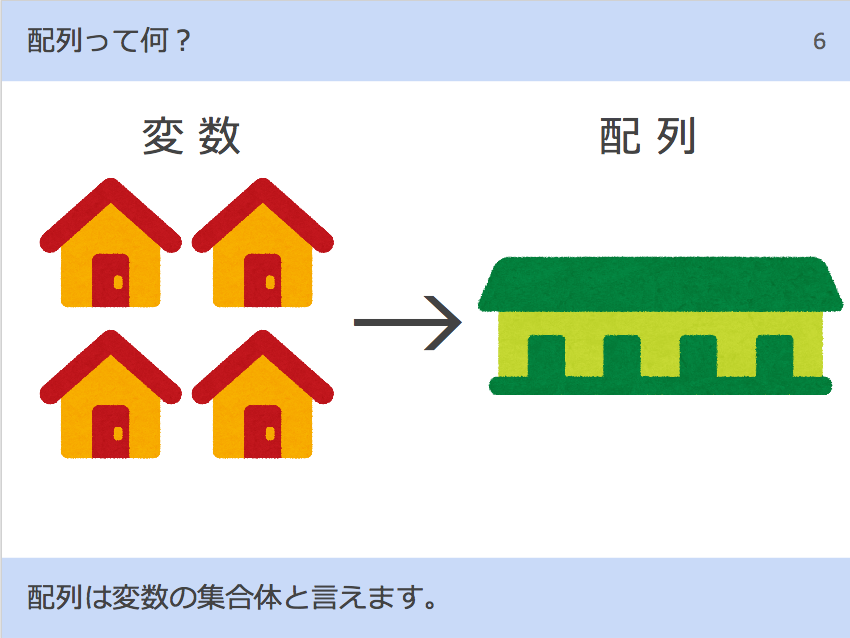
\includegraphics[width=10cm, bb=0 0 850 638]{img/9thParagraph/gainen_01.png}
\end{center}
\caption{概念スライド}
\end{figure}

\bunseki{新保遥平}

\subsection{例題}
例題の部分ではまず、図9.2のように例題のソースコードをユーザーに見せて、このソースコードがどのように動くのかを考えさせる。これよって、次の画面でユーザーが頭の中で考えていたソースコードの動きが合っているかを確認することができる。また、この例題の部分もGoogleスライドを用いて作成した。

\begin{figure}[H]
\begin{center}
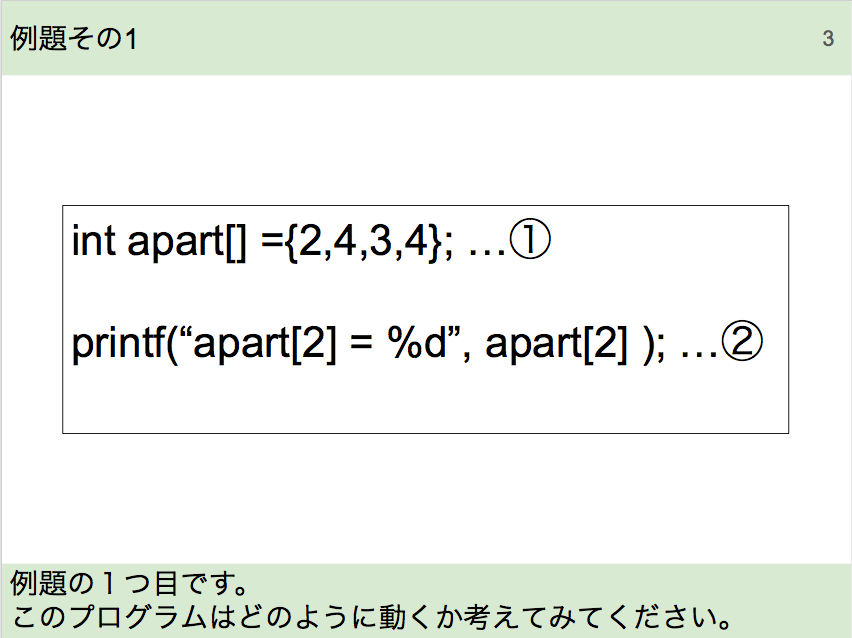
\includegraphics[width=10cm, bb=0 0 852 638]{img/9thParagraph/reidai_01.png}
\end{center}
\caption{例題スライド1}
\end{figure}

次に図9.3、図9.4のようにアパートとソースコードを組み合わせて説明を行う。具体的には、1行目のソースコードではapart[0]には住人が2人、apart[1]には住人が4人、apart[2]には住人が3人、apart[3]には住人が4人が未来アパートに住んでいることをアニメーションで説明している。次に2行目のソースコードではapart[2]の表示を行うことを示している。また、ソースコードが示している部分がアパートのどのような状態かを合わせて説明している。これによって、ユーザーがソースコードの動きを見ながら配列を理解することができると考えた。

\begin{figure}[H]
\begin{center}
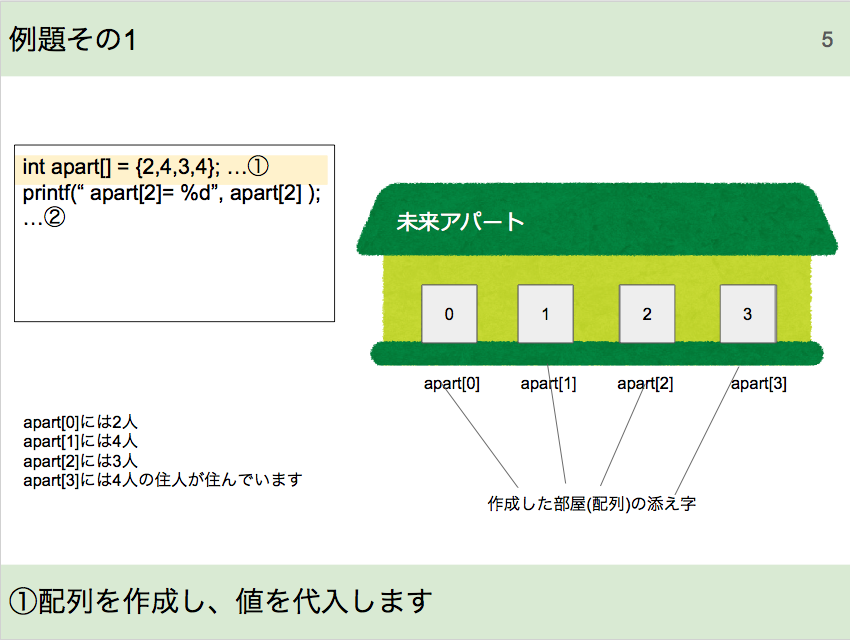
\includegraphics[width=10cm, bb=0 0 850 640]{img/9thParagraph/reidai_02.png}
\end{center}
\caption{例題スライド2-1}
\end{figure}

\begin{figure}[H]
\begin{center}
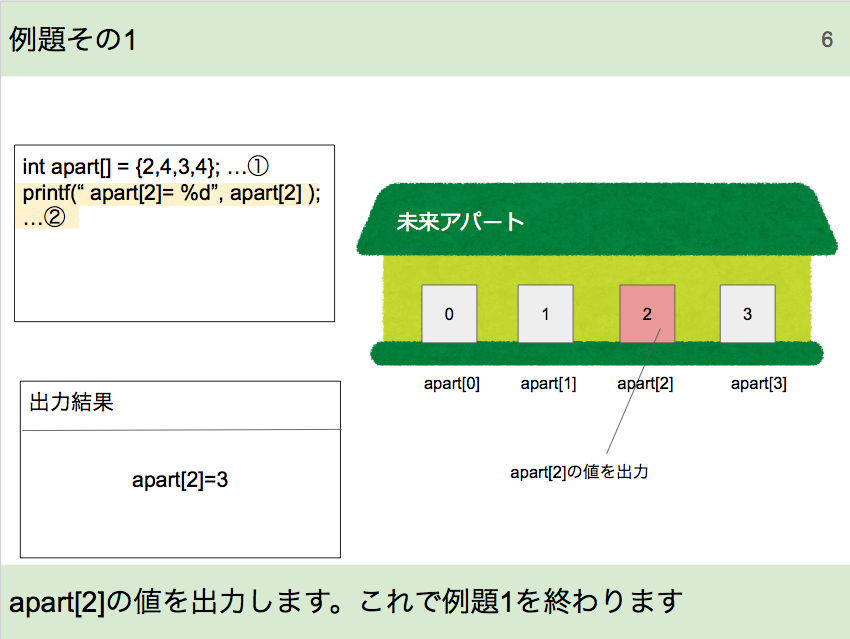
\includegraphics[width=10cm, bb=0 0 850 639]{img/9thParagraph/reidai_03.png}
\end{center}
\caption{例題スライド2-2}
\end{figure}

\bunseki{新保遥平}

\subsection{確認問題}
確認問題ではインタラクティブな学習を行ってもらうために、図9.5、図9.6のように、実際にユーザーに値を入力をして問題を解いてもらうことを目的とした。また、この確認問題の工夫した点は配列の値をランダムにし、ユーザが飽きないように何回も学習することができ、入力した値によってアニメーションが変化するところである。


\begin{figure}[H]
\begin{center}
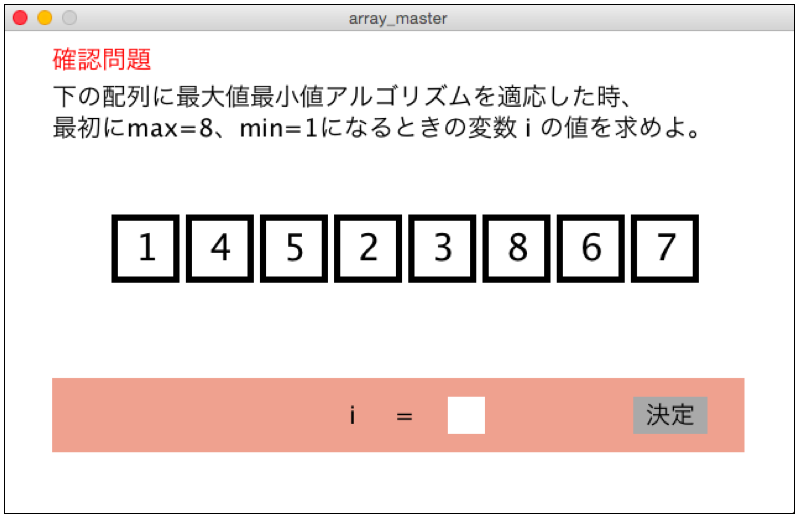
\includegraphics[width=10cm, bb=0 0 798 516]{img/9thParagraph/kakuninmondai_01.png}
\end{center}
\caption{確認問題 入力画面1-1}
\end{figure}

\begin{figure}[H]
\begin{center}
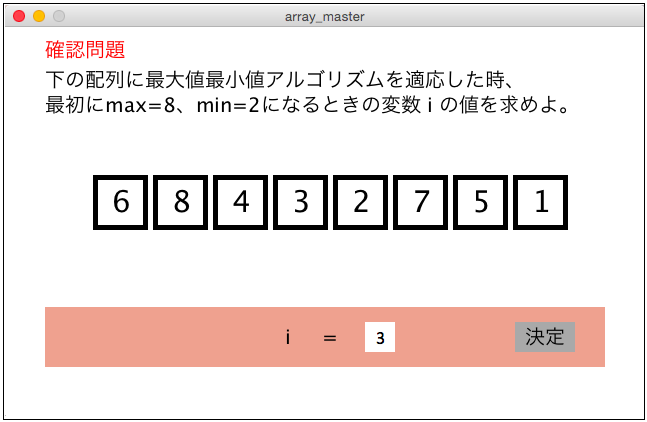
\includegraphics[width=10cm, bb=0 0 647 422]{img/9thParagraph/kakuninmondai_02.png}
\end{center}
\caption{確認問題 入力画面1-2}
\end{figure}

ユーザーには図9.7、図9.8のように確認問題のソースコードを見ながら確認問題を解いてもらう。この確認問題は未来大の1年生が「プログラミング基礎」の授業で扱う講義スライドを参考に我々が考えた問題である。問題の内容は、与えられた配列に入った8つの値の指定された大小の値を求めるときの繰り返す回数を考えさせるものである。流れとしては、ユーザーが答えだと思う値をキーボードから入力する。

\begin{figure}[H]
\begin{center}
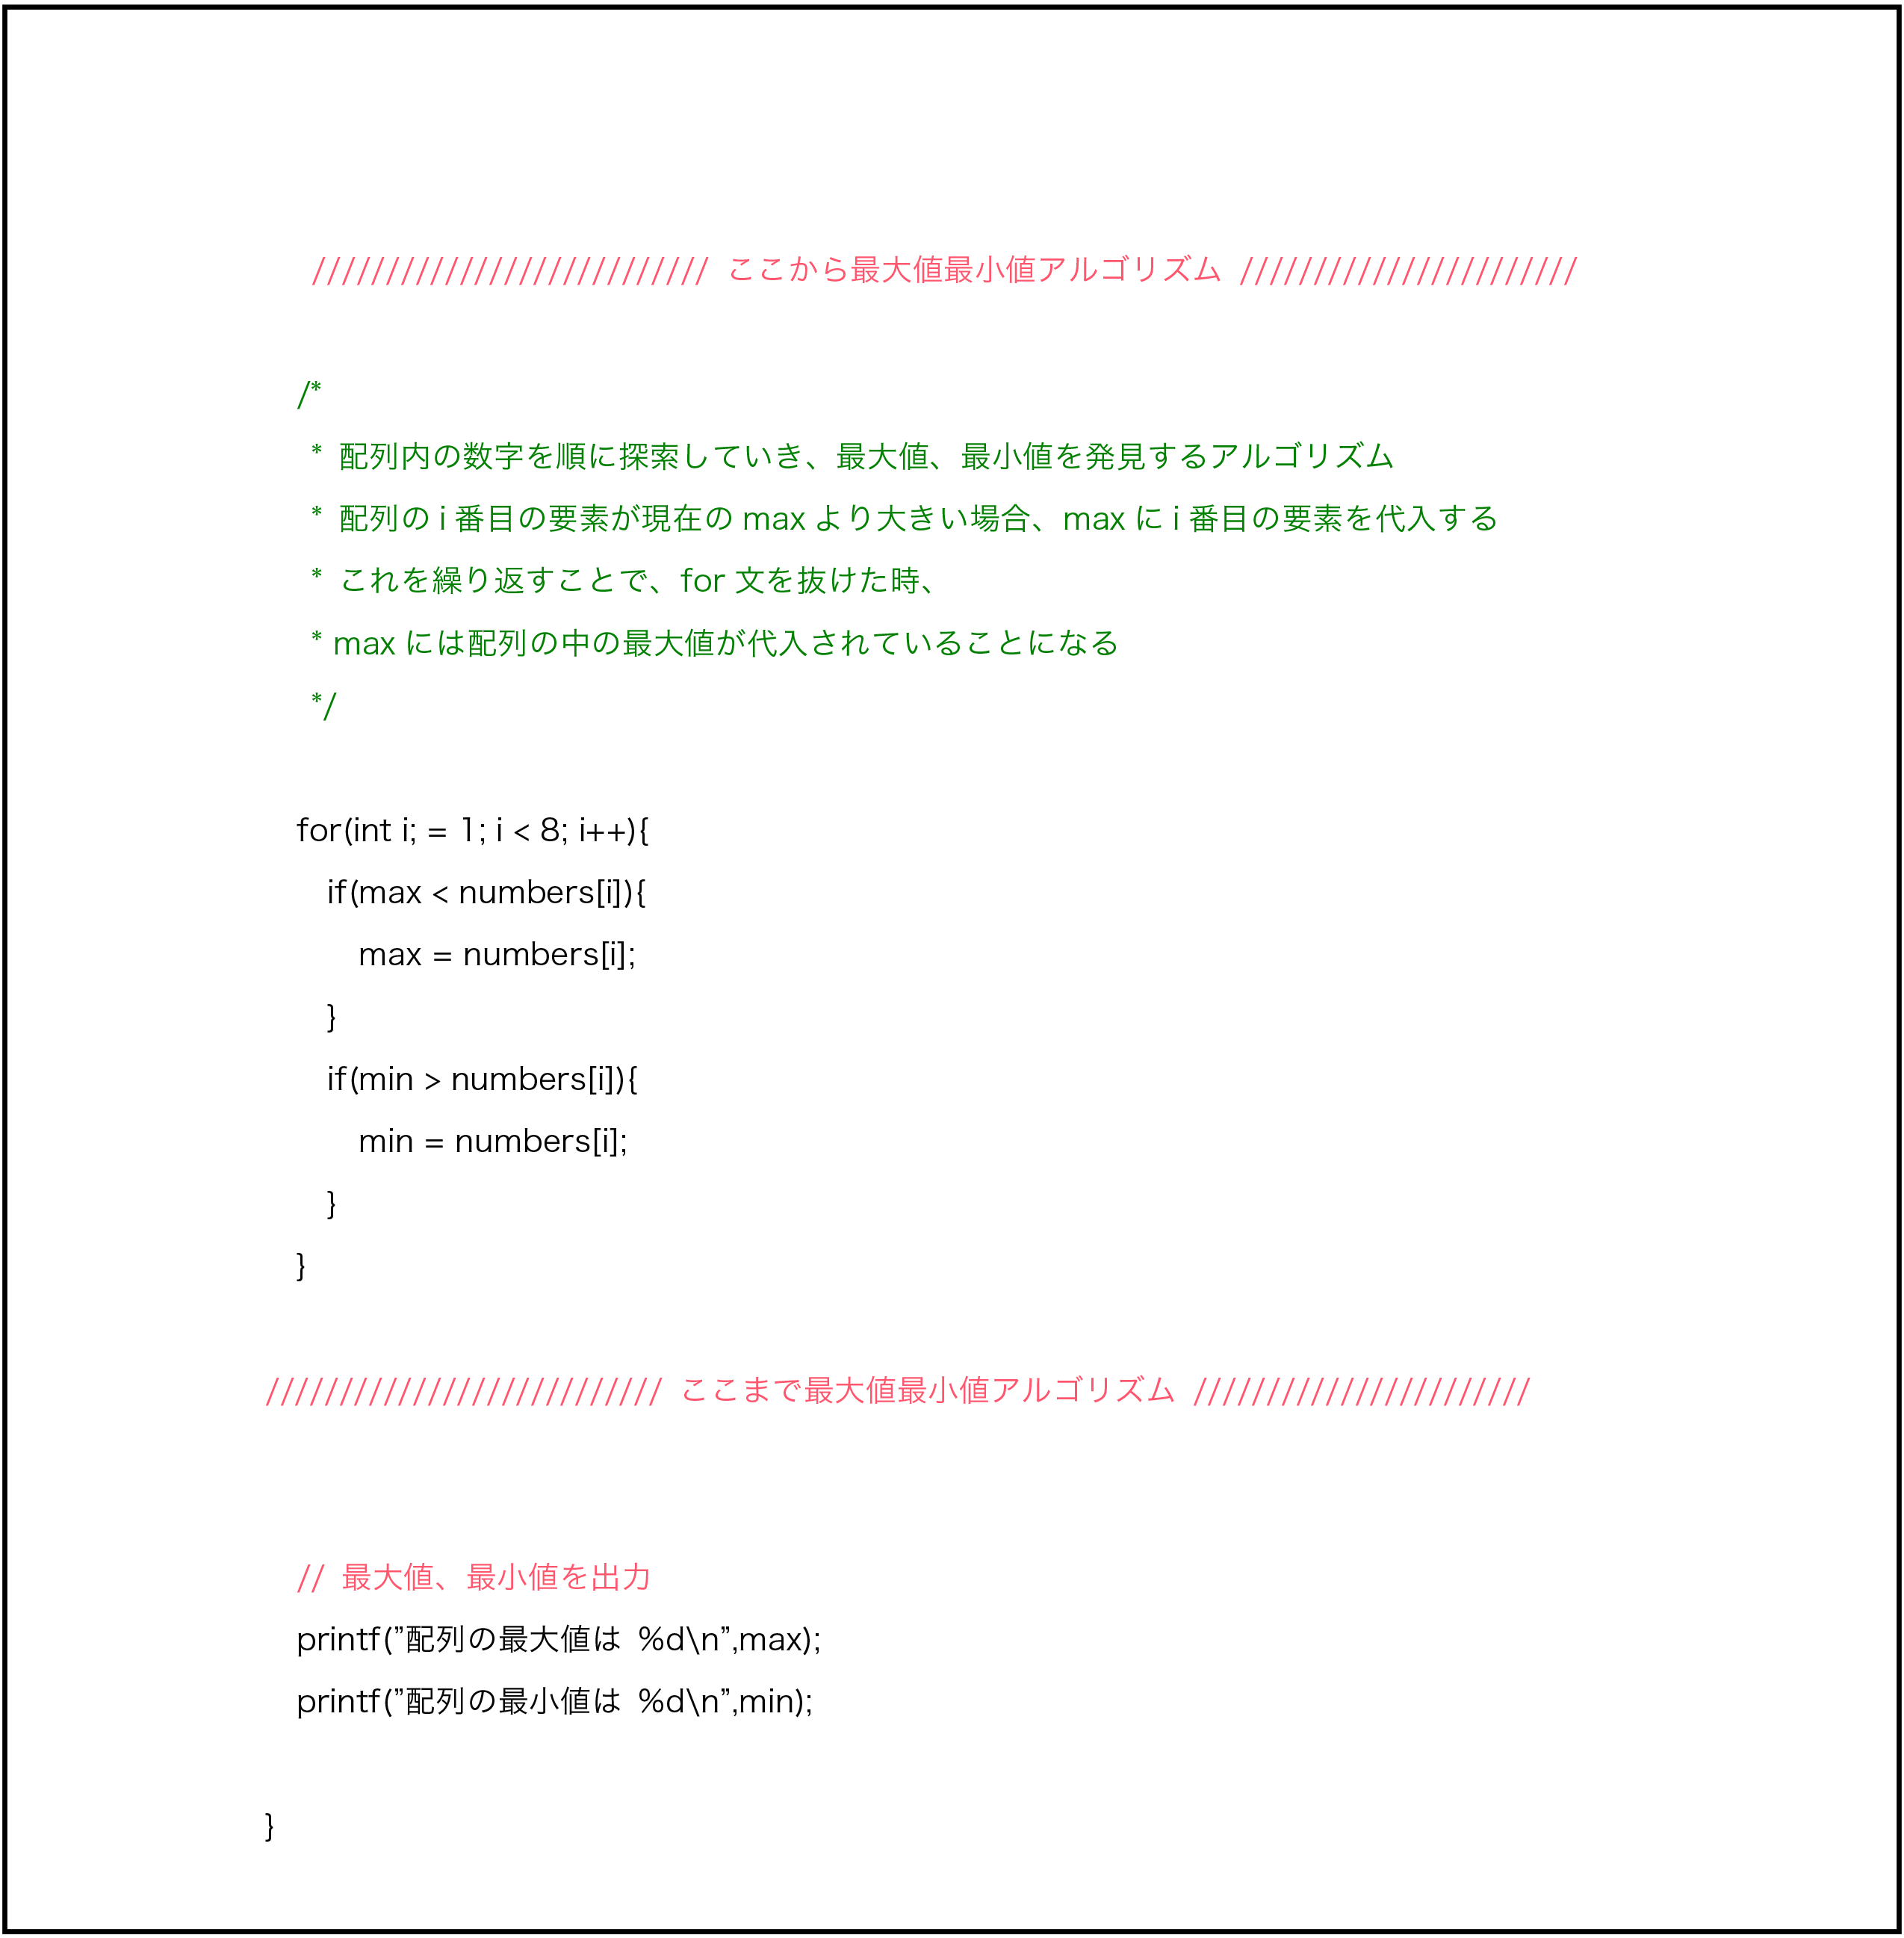
\includegraphics[width=14cm, bb=0 0 2549 2594]{img/9thParagraph/kakuninmondai_03.png}
\end{center}
\caption{確認問題 ソースコード1-1}
\end{figure}

\begin{figure}[H]
\begin{center}
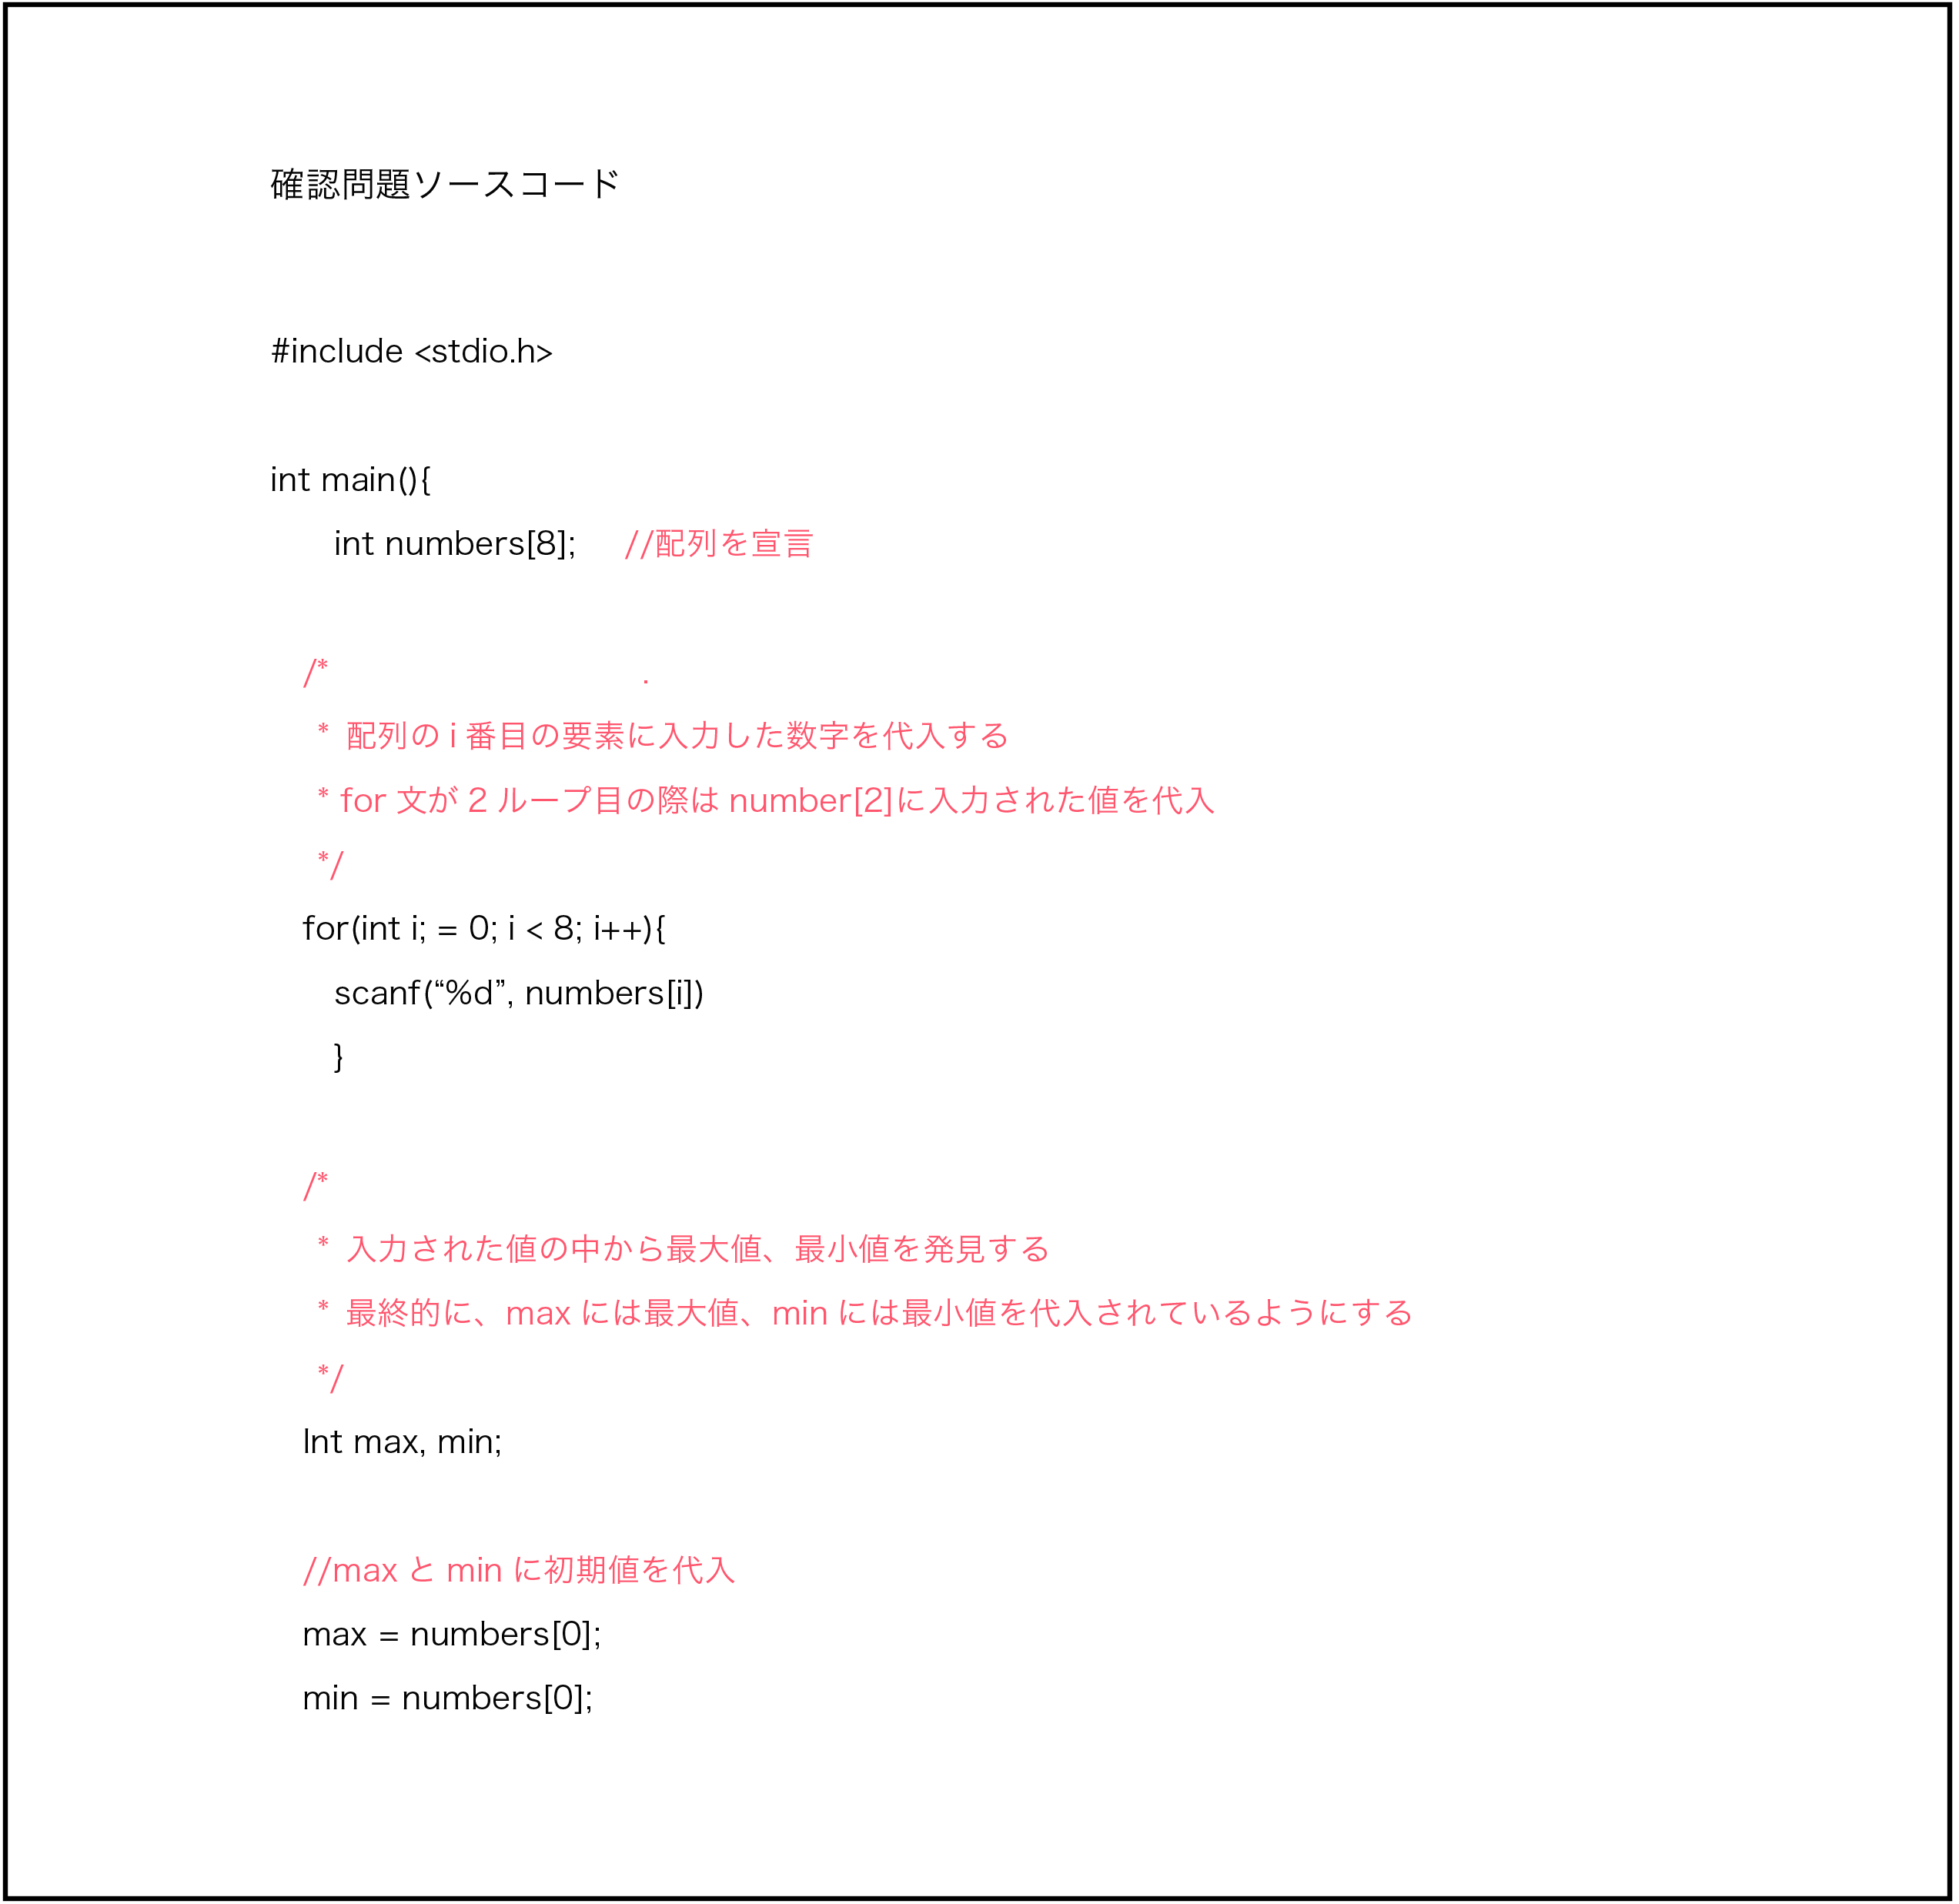
\includegraphics[width=14cm, bb=0 0 2545 2474]{img/9thParagraph/kakuninmondai_04.png}
\end{center}
\caption{確認問題 ソースコード1-2}
\end{figure}

すると、図9.9、図9.10のように入力した値が正しいか、間違いかをすぐに表示する。そして入力した値が間違っている場合、その後プログラムがどうなるかを説明する。これは、ユーザーがなぜ「この値が間違っているのか」を理解してもらうためである。このようにして、確認問題でユーザーが本当に配列を理解したのかを確かめている。


\begin{figure}[H]
\begin{center}
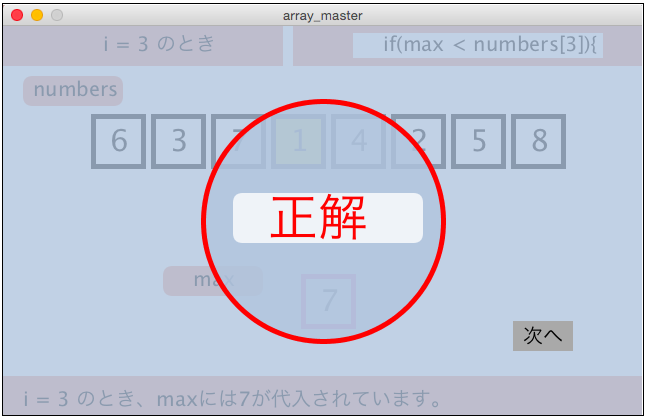
\includegraphics[width=10cm, bb=0 0 645 418]{img/9thParagraph/kakuninmondai_05.png}
\end{center}
\caption{確認問題 正解画面}
\end{figure}

\begin{figure}[H]
\begin{center}
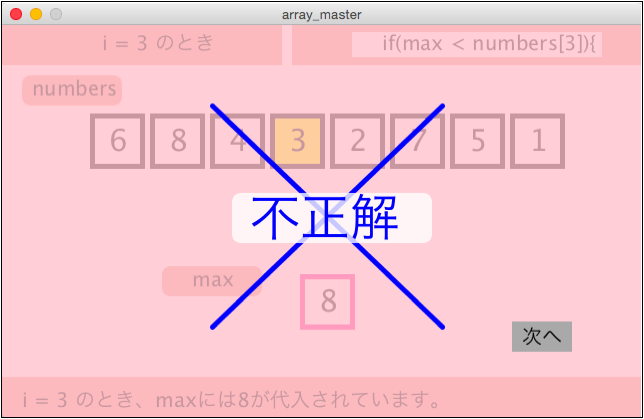
\includegraphics[width=10cm, bb=0 0 644 419]{img/9thParagraph/kakuninmondai_06.png}
\end{center}
\caption{確認問題 不正解画面}
\end{figure}

\bunseki{新保遥平}

%10章
%%%%%%%%%%%%%%%%%%%%%%%%%%%%%%%%%%%%%%%%%%%%%%%%%%%

\chapter{後期の結果}

\section{プロジェクトの評価}
\par 12月に行われた最終発表の評価シートの結果から「声が大きく、ポスターが見やすかった」、「円滑に話を進めており、聞き取り易い」、「具体的な説明をしながらデモができてた」などの意見をいただき、前期の中間発表と同様に発表技術は高い評価を得られた。一方、発表内容に関しては「アプリ内容が分かり易く、教育アプリは使えると思いました」、「イメージがわくので、分かり易かったです」、「前期と後期のつながりが分かり易く説明されていた」などの意見をいただき、後期と比べ高い評価をいただいた。また、「実際に1年生に使ってほしかった」、「教育アプリが他の班と比べて劣って見えた」、「他の班と比べてiOSアプリを作らなかったメリットを知りたい」などの意見をいただき、自分たちの活動の不十分な点を知ることができた。
\par これらのことから、後期のプロジェクトは前期と比べて第三者の方に伝えられる内容であったと思われる。また、改善する必要がある部分を知ることができたため、それらを改善していきたいと思う。
\bunseki{中進吾}

\section{プロジェクトの成果}
\par 後期の活動の成果は以下の2点である。
\begin{itemize}
\item 前期は、活動時間を無駄にすることが多く何度も居残りをしていた。後期はそれを防ぐために、プロジェクトが始まる前にグループリーダーがLINEでメンバーに今日のアジェンダを伝えた。その結果、メンバー全員がその内容を意識して話し合いを行ったことで、活動の時間を無駄にすることがほとんどなくなった。このことから、活動を始める前に話す内容を伝えることは重要なことだということがわかった。
\item 
本プロジェクトは中間発表、アカデミックリンク、最終発表の3つの発表会に参加し、いずれもポスターセッションで行った。3度の発表会を経験した結果、最初はメンバーの数人しか発表することができなかったが、最終発表会ではメンバー全員が人前で発表することができるようになった。今後、研究成果発表など発表の機会は多く存在するため、メンバー全員が人前で堂々と発表できるようになったことは、大きな成果だと思われる。
\end{itemize}
\bunseki{中進吾}


%11章
%%%%%%%%%%%%%%%%%%%%%%%%%%%%%%%%%%%%%%%%%%%%%%%%%%%

\chapter{今後の課題と展望}
\section{開発アプリの課題と展望}
最終発表会を終えてから、TAから本グループの開発アプリに酷似したソフトウェアが本学の2年次の科目である「アルゴリズムとデータ構造」の教科書の付属CDにあるという意見を頂いた。その中身は、プログラムの実行に伴って、刻々と変化するプログラムの流れや変数などを、C言語で書かれたプログラムリストと対比しながら、視覚的に体験学習できる「アルゴリズム体験学習ソフトウェア」である。その中に三値の最大値を求めるプログラムがあり、アニメーションの速度を調整できたり、変数の初期値を変更することや1コマづつ動かすことも可能になっている。本グループの開発アプリにはない機能や似たような機能が入っていることを踏まえ、これからグループで検討すべき課題である。

\par
「アルゴリズム体験学習ソフトウェア」には、ユーザの入力によってアニメーションが変化するなどの相互作用がないため、本開発アプリでは今ある機能だけではなく、教育性を高めるためにユーザとアプリの相互作用が高い機能をつける。また、現状の開発アプリは、配列のアニメーションしか作成していなく、コンテンツとしては不十分である。そのため、配列に加えて、ポインタ、構造体などの1年生が難しいと感じる単元を調査し、アニメーションを加え、Webアプリケーションとしての体裁を整えていく。その後、本学の1年生に開発アプリを使って評価を行い、アプリを改善していく。

\par
また、最終発表会で「メタ学習センターと連携してみては?」という意見を頂いた。本プロジェクトの最終目標である未来大学の授業の予習、復習用の教材として使ってもらうだけではなく、メタ学習センターと連携しプロジェクト学習、メタ学習センター、授業が連携して学生に教育できるようになることが今後の展望である。


\bunseki{皀勢也}

\section{メンバーの課題と展望}
前期の活動では、中間発表会に向けて、プロトタイプを制作する実装班と、ポスターを制作するポスター班で分かれたが、いくつか課題があった。アプリやポスターに使われる画像の制作は情報デザインコースのメンバーがほとんど一人で作っていたため、実装がスムーズにいかなかった。なるべくタスクをメンバーで分散させるべきであった。また、ポスター班は実装に関わっていなかったため、実装班とのスキルの差があった。
\par
また、アプリ案を決める際に本プロジェクトメンバー、TA、担当教員に毎回アプリ案の発表を行っていた。そこで頂くレビューに対し、グループメンバー誰一人しっかりとした説明や対案をすぐに示すことができなかった。そのためレビュー内容の修正をするではなく、要件定義、設計をやり直すことを何度も行っていた。
\par
さらに、プロジェクト学習の授業外での作業が多く、メンバー全員が作業できない日があった。そのため、情報共有に時間がかかったり、効率良く作業をすることができなかった。
\par
後期の活動では、最終発表会に向けて概念の説明、例題、確認問題を制作する実装班とポスターのデザインを考え、制作するポスター班、Webサイトのレイアウトやロゴを決めるWeb班に分かれて活動を行った。確認問題を制作するにあたって、残っている実装期間を考え1年生の頃に使用し慣れているProcessingを用いて、実装を行った。その結果、新しい言語であるSwift言語を習得することができなかった。また、ほとんど一人のメンバーがProcessingで実装を行っていたため、コード規約がなく他のメンバーが理解するのに時間がかかるコードになってしまった。
\par
また、プロジェクト時間外に進捗報告をする機会がなかったため、メンバーが何の作業をしているか把握できずにメンバーのタスクの量に偏りが発生した。さらに、グループでの話し合いに時間をかけすぎてしまうことや、論点にずれが生じメンバーの共通認識に相違が発生してしまうことが多くあった。
さらに、Web班をメンバー1人に任せていたことやオンラインクラウドストレージに保存し、グループメンバーで進捗確認を行っていなかったため、Webサイトのレイアウトを構築を行っていたメンバーが作業データを紛失してしまい、スケジュールが大幅に遅れてしまったことがあった。

\par
今後の展望は、メンバーの役割を適切に決めることや進捗確認を毎日行うなどし、お互いの進捗を確認し、タスクの量に偏りがないかを適宜確認する。また、活動を行う前には活動計画を決めることや話し合いの際には、時間を決めファシリテーターを設定し、論点がずれていないか客観的に見るようにしていく。また、グループメンバー全員が開発アプリに対して共通認識を持ち、適切な説明ができるようになることである。

\bunseki{皀勢也}


%12章
%%%%%%%%%%%%%%%%%%%%%%%%%%%%%%%%%%%%%%%%%%%%%%%%%%%

\chapter{学び}
\section{グループとしての学び}
本グループでは、前期と後期の活動が異なり失敗を多く経験してきた。以下の4点が失敗から特に学んだことである。
\begin{itemize}
\item 
想定外のタスクが発生した際に、先の見通しを立てることができず、作業時間を無駄にした。このことから作業の変更や遅れが発生したとき、随時スケジュールの更新を行うことで効率よく作業を行うことの重要性を学んだ。

\item 
話し合いに時間をかけすぎてしまい議題が少しずつ脱線し、議論に集中できなくなって議論についていけなくなったメンバーがいたり、メンバー全員で最終的な議論の共有ができていなかった。そのため、作業の遅れが発生した。このことから活動する前に活動計画を決めることや話し合いの時には時間を決め、議論が正しい方向で進んでいるか客観的に見ることの重要性を学んだ。

\item
前期ではアプリ案の要件定義を固めずに実装を行ったため、目的と提案が噛み合っていなく、一貫性がない内容が分かりにくい提案となってしまったことや教育系グループとして教育という意味をしっかり決めていなかったため、何度も提案内容の変更があった。このことから課題調査を深く行い、設計をしっかり行うことの重要性を学んだ。

\item
プロジェクト学習の授業外での作業が多く、議事録を残していないことがあり、情報共有がうまくできていなかった。さらに進捗確認をきちんと行っていなかったため、メンバーが何をしているのか把握できずにメンバーのタスクの量に偏りが生じた。このことからメンバーの役割を適切に決めることやタスク看板を用いることでお互いの進捗を確認し、情報共有することの重要性を学んだ。

\end{itemize}
\par
前期での失敗を後期で振り返ることで、後期の活動をスムーズに行うことができた。開発アプリの目標は達成することができなかったが、多くの経験や学びを得ることができたため、プロジェクト学習としての目標は達成できた。

\bunseki{皀勢也}

\section{各メンバーの学び}
\subsection{熊谷優斗}
\par これまで大学での活動の中で何度かPBLは経験したものの、自ら課題を考え主体的に活動したことは初めての経験だったため、様々な学びを得ることができた。その中でも、今回は2つの学びをとりあげる。1つ目の学びは、メンバーに技術を教えることの難しさだ。過去のPBL経験から、Gitに関しての知識は持っていたため、メンバーにGitとGitHubの使い方を教える役目を受け持った。しかし、メンバーによって理解度の差があるにも関わらず、理解できているメンバーに合わせて話を進めていってしまった。そのため、メンバー全員にGitの使い方を理解してもらうことができなかった。このことから、メンバーの理解状況を確認し、全員が理解した上で次のステップに進む、という教え方が大切であることを学んだ。2つ目の学びは、適切な文言を使用することの重要性だ。前期の活動では、「基本的な制御文の書き方を学ぶ」という意味で、「簡単なアルゴリズムを学ぶ」という文言を使用していた。その結果、TAや教員によるレビューの際に、自分たちが作成したいアプリケーションの内容をうまく伝えることができず、苦労した。このことから、適切な文言を使用することは、他人に自分の意見を伝えるために重要であることを学んだ。
\bunseki{熊谷優斗}

\subsection{皀勢也}
前期は本プロジェクトを進めるにあたって、Swift言語を使ってプログラミングを行うためXcodeが入っているMacOSが必要であった。自分はWindowsのノートパソコンしか持っていなかったため、enPiTからMacBook Airを借りて作業を行った。初めは、Windowsと異なり上手く作業を進めれなかったが、使っているうちにMacOSに慣れて上手く作業できるようになった。
\par
また、グループで開発を行っていくうちに、他者にもわかりやすいソースコードを書くように意識した。さらに、GitとGitHubを使ってバージョン管理することや議事録を残すことの重要性を学んだ。
\par
本グループのメンバーにはICT演習に参加しているメンバーと情報デザインコースに所属しているメンバーがいたため、話し合いの進め方や要件定義プロセスなどの様々な技術と知識を吸収することができた。そのため、他にグループ活動をするときは自分がリーダーとなって活動を進めていくことができるようになった。
\par
後期では、Processingを用いて実装を行ったことに加え、スライドを作って企業講師にグループの活動を発表したり、ポスター制作を行った。プロジェクトが始まった当初は、発表経験があるメンバーに発表を任せていたため、発表の技術がうまくならなかった。後期から人前で発表することや、話し合いに積極的に参加することで人に伝える技術が身についた。またポスター制作などでメンバーやTAからレビューを頂き、修正をスムーズに行うことができた。この経験からレビューの重要性を学び、積極的にレビュー行うようになった。

\bunseki{皀勢也}

\subsection{新保遥平}
\par この1年間では多くのことを学んだ。技術的な点では主に3つの学びを得た。1つめにGitHubをしっかりと理解して使えるようになったことだ。GitHubは以前に使ったことがあったが、曖昧な部分が多くわからない部分も多くあった。だが、プロジェクトが始まってからはグループ内でもGitHubを上手く使ってアプリの開発や報告書の作成を行うことができた。2つ目に、ポスターの作成のためにAdobe Illustratorの使い方を学ぶことができた。他プロジェクトではポスターの作成はデザインコースの人が作るプロジェクトが多い中、自分もポスター作成に携わることができ、いい経験になった。3つ目は発表技術である。私は即席で人の前で話すことがとても苦手であったが、この一年、何度も即席で話す機会が多くあり、自分の意見をまとめて話すことができるようになった。

\par 前期は自分一人で行うべきでないタスクも一人で行ってしまったため、自分のタスクの進捗が遅れることがあった。このことから、プロジェクトリーダーとして、人に仕事を振リ分けることの重要性を学んだ。

\par また後期は、プロジェクトが始まる前に今日の活動のアジェンダ、終わる際に、今日の進捗報告を行った。これは各グループの活動が不透明だったからである。実際に開発しているアプリの進捗を聞くことによって他のグループからの相互レビューを受け、アプリ案の修正を行うことができた。このことから、プロジェクトリーダーとして情報共有の重要性を学んだ。

\bunseki{新保遥平}

\subsection{中進吾}
\par 私がこのプロジェクト学習で学んだことは以下の4つである。
\par 1つ目は、メンバーに仕事を均等に振り分けることができていなかったため、進捗が遅れることがあった。このことから、メンバー1人を頼りすぎてしまうとスケジュールが遅れてしまうことが分かった。
\par 2つ目は、私はこれまでに2度PBLに参加してきたが、要件定義は先輩に任せて自分は実装ばかりを行っていた。今回、一から要件定義を考えたことは大きな学びであり、自分に足りないものを見つけることができた。今後、PBLに参加するときには自分から率先して要件定義を立て、この経験を後輩に伝えていきたいと思う。
\par 3つ目は、後期は、今日のアジェンダをメンバー全員に伝え、時間の管理を行った結果、前期と比べプロジェクトをうまく進めることができた。アジェンダを流すこととタイムマネジメントをすることの重要性を知ることができた。
\par 4つ目は、毎回のプロジェクト学習の終了前、進捗報告を行っていた。そのため、チーム全体が今日何をやってどこまで進んだのか、メンバー全員で共有することができた。このことから、進捗報告の重要性を学ぶことができた。
\bunseki{中進吾}

\subsection{矢吹渓悟}
デザインプロセスの大切さを再認識し、同時に自分の未熟さを痛感した。なぜなら、初期テーマの設定からブレインストーミングやフィールドの調査を怠ってしまったからだ。本来ならば、メンバーが一丸となって、話し合いや現状を調べながら、みんなでテーマを確立するべきだ。しかしながら、今回は個人個人がやりたいものを考え、そこから一つに絞ってしまったのだ。そのため、背景情報や対象ユーザーの設定が偏見や想像論になったり、後付けとなり、プロジェクトの根幹が揺らいでしまい、最終的にテーマの見直しまでに落ちてしまった。よって、今後テーマを見直す上で大切なのは、ブレインストーミングなどを通していろいろな可能性を吟味した上で、徐々に一つに絞り込むことが大切だと再認識した。
\bunseki{矢吹渓悟}




% 以降、付録(付属資料)であることを示す
\begin{appendix}

\chapter{新規習得技術}
\par【Swift】
\par《キーワード》
\par Swift・Xcode・SpriteKit・iPhone・iPad・Mac・オブジェクト指向・iOSアプリケーション
\par《概要》
\begin{itemize}
\item 2014年にWWDCで発表された、新しいオブジェクト指向型のプログラミング言語
\item Objective-Cに代わるiOSアプリケーション開発言語
\item 開発環境はMac、実機テスト用にiPhoneやiPadが必要で、開発エディタはXcodeが推奨される
\item 開発する上で、iOS Developer Programへの登録が必要
\item SpriteKitという2Dカジュアルゲーム用のフレームワークなど、幾つかテンプレートが用意してある
\end{itemize}
\par《Swiftの特長》
\begin{itemize}
\item 速い:Objective-Cより実行速度が高速
\item モダン:プログラミングの書き方が新しい
\item 安全:プログラミングにエラーが起きにくい仕組みが増える
\end{itemize}
\par《Objective-Cとの主な相違点》
\begin{itemize}
\item 行末のセミコロンや制御文の()が不要
\item メソッドの記述方法が「.メソッド名()」と一般的な記述に
\item 変数にnilが代入されるとエラーが表示され、安全性が向上した
\item 別クラスにアクセスするときもimportが不要
\end{itemize}
\par《Xcodeとは》
\begin{itemize}
\item iPhoneアプリを作るための開発ツール
\item アプリを作るのに必要な作業を全て行う
\end{itemize}
\par(ex:アプリ画面のデザイン・プログラムの入力・実行ファイルの作成)
\begin{itemize}
\item iOSシュミレーターで実機を使わなくても粗方のデモストレーションが行える
\end{itemize}
\par《SpriteKitを使うメリット》
\begin{itemize}
\item 文字やグラフィックスを素早く表示させたり動かしたりすることができる
\item 2Dの物理エンジンがついているため、物理的な動きをシュミレートさせることができる
\end{itemize}

\par【Git / GitHub】
\par《キーワード》
\par Git・GitHub・分散型・バージョン環境システム・リポジトリ・ローカル・保存(コミット)・オープンソース
\par《概要》
\par[Git]
\begin{itemize}
\item プログラムソースなどの変更履歴を管理する、分散型のバージョン管理システムのこと
\item Linuxの開発チームが使用していたことがきっかけとなり、徐々に世界中に広まった
\end{itemize}
\par[GitHub]
\begin{itemize}
\item Gitの仕組みを利用して、世界中の人々が自分の作品(プログラミングコードやデザインデータ、ドキュメントなど)を保存・公開することができるウェブサービスのこと
\item 運営はGitHub社で、個人・企業を問わず無料で行うことができる
\item 基本的にオープンソースだが、有料サービスを利用するとプライベートなリポジトリも作ることができる
\end{itemize}
\par《Gitと従来品の比較》
\par[Git]
\begin{itemize}
\item 自分のパソコンなどのローカル環境に、全ての変更履歴を含むリポジトリが複製される
\item 各ローカル環境がリポジトリのサーバーとなれる
\item ローカル環境にもコードの変更履歴を保存(コミット)できるので、リモートのサーバーに接続する必要がない
\item ネットワークに接続していなくても作業ができる
\end{itemize}
\par[従来]
\begin{itemize}
\item サーバー上にある一つのリポジトリを共同で使っていた
\item 利用者が増えると変更内容の衝突が頻繁に起きる
\item 整合性を維持するのが大変
\end{itemize}


\chapter{活用した講義}
%\begin{hissu}
\par【情報デザイン1】
\par《キーワード》
\par Adobe Illustrator・図解表現・ポートフォリオ
\par《授業内容》
\begin{itemize}
\item Adobe Illustratorの使い方(個人)
\item 市立函館博物館を題材とした図解表現(個人)
\item 図解表現の説明も兼ねたポートフォリオの作成
\end{itemize}
\par《活かせる技術・知識・経験》
\begin{itemize}
\item 画像やアプリ素材をAdobe Illustratorで作成すること。
\item 議事録や発表ポスターの素材を図解を用いて表現すること。
\end{itemize}

\par【情報デザイン2】
\par《キーワード》
\par グループワーク・タンジブル・アクティングアウト(寸劇)・プロトタイピング・ストーリーテーリング・プレゼンテーション・ポートフォリオ・図解
\par《授業内容》
\begin{itemize}
\item 時計の分析(グループ)
\item スマートウォッチの分析(グループ)
\item タンジブルな提案(グループ)
\end{itemize}
\par《活かせる技術・知識・経験》
\begin{itemize}
\item 机に座って話し合いするよりも、手足を動かして考える方がより良い提案になること。
\end{itemize}

\par【情報表現基礎3】
\par《キーワード》
\par グループワーク・観察・フィールドワーク・アクティングアウト(寸劇)・プロトタイピング・ストーリーテーリング・スケージューリング・プレゼンテーション・ポートフォリオ・図解
\par《授業内容》
\begin{itemize}
\item カバンのスケッチを通した観察(個人)
\item オートマタ制作(個人)
\item 西部地区のフィールドワークを通して、より西部地区に足を運べる物・事・企画の提案(グループ)
\item 各ポートフォリオの作成
\end{itemize}
\par《活かせる技術・知識・経験》
\begin{itemize}
\item 情報共有をしっかりと行わないと、メンバー間の考えのズレやタスクの進捗に影響すること。
\item 提案のユーザーストーリーを考えて、提案がユーザーにどういう変化を与えるのかを常に考えながら、作成していくこと。
\item 提案をプロトタイピングし、デモストレーションやアクティングアウトなどを行う。それを通して、問題点・優良点・改善点などを発見しやすくすること。
\item プレゼンテーションにアクティングアウト(寸劇)や提案のデモストレーションを盛り込んで、発表に説得力を持たせること。
\end{itemize} 


%\chapter{相互評価}
%\begin{hissu}
%課題解決過程で分担し、連携した作業全般について、互いに客観的に評価する。 
%\end{hissu}

%\chapter{その他製作物}
%\begin{hissu}
%その他成果物をプロジェクトの担当教員の指示に従って添付する。
%\end{hissu}

%付録の終わり
\end{appendix}


%\backmatter

% 参考文献
\begin{thebibliography}{9}
% \bibitem {ラベル} 著者名. 書籍名. 出版社,  年号.
% \bibitem {A2} ほげほげお. うんたらかんたら,  2003.
 \bibitem {A2} Code部. 5歳からプログラミング必修化!?世界の最新IT教育トレンドまとめ |Code部,  2015. \url{http://blog.codecamp.jp/programming_education/} (2015/7/20)
 \bibitem {A2} TechAcademy. プログラミングが義務教育に!政府の成長戦略素案に盛り込まれたプログラミング教育の内容とは |TechAcademyマガジン,  2013. \url{http://techacademy.jp/magazine/736} (2015/7/20)
  \bibitem {A2} Code部. 大人も子供も楽しめる!プログラミング入門ゲーム「Scratch」をやってみた|Code部 ,  2015. \url{http://blog.codecamp.jp/try_scratch/} (2015/7/20)
 \bibitem {A2} 日本経済新聞. 中学の技術・家庭科で「ビジュアルプログラミング」を導入:日本経済新聞,  2012. \url{http://www.nikkei.com/article/DGXNASFK2701H_X21C12A2000000/} (2015/7/20)
 \bibitem {A2} ヴィストン株式会社. 計測器プログラマー |ヴィストン株式会社,  2012. \url{http://www.vstone.co.jp/products/mcprogrammer/} (2015/7/20)
  \bibitem {A2} コードアカデミー高等学校. コードアカデミー高等学校,  2015. \url{http://www.code.ac.jp/} (2015/7/20)

  \bibitem {A2} 生活総研ONLINE. 生活定点1992-2014,  2014. \url{http://seikatsusoken.jp/teiten2014/} (2016/1/11)

\end{thebibliography}

\end{document}